\documentclass[11pt, a4paper,polish,twoside]{report}
\usepackage{graphicx}
\usepackage{times}
\usepackage[T1]{fontenc}
\usepackage[polish]{babel}
\usepackage[utf8]{inputenc}
\usepackage{lmodern}
\usepackage{hyperref}
\usepackage{graphicx}
\usepackage{pdfpages}
\usepackage{mathtools}
\selectlanguage{polish}
\usepackage{indentfirst}
\usepackage{gensymb}
\usepackage{rotating}
\widowpenalty=10000
\pagestyle {plain}
\usepackage{float}
\usepackage{geometry}
\usepackage{mathptmx}
\newgeometry{tmargin=2.5cm, bmargin=3.0cm, left=3.5cm, right=2.5cm}
\setcounter{secnumdepth}{2}
\linespread{1.3}
\usepackage{etoolbox}
\patchcmd{\chapter}{\thispagestyle{plain}}{\thispagestyle{fancy}}{}{}
\setlength{\headsep}{1.5cm}
\usepackage{listings}
\usepackage{lastpage}
\usepackage[MeX]{polski}
\graphicspath{ {./pictures/} }
\newcommand{\HRule}{\rule{\linewidth}{0.5mm}}
\usepackage{fancyhdr}
\pagestyle{fancy}
\setcounter{tocdepth}{1}
\usepackage[backend=bibtex]{biblatex}
\bibliography{bibliografia.bib}

\lstdefinelanguage{JavaScript}{
  keywords={typeof, new, true, false, catch, function, return, null, catch, switch, var, if, in, while, do, else, case, break},
  keywordstyle=\color{blue}\bfseries,
  ndkeywords={class, export, boolean, throw, implements, import, this},
  ndkeywordstyle=\color{darkgray}\bfseries,
  identifierstyle=\color{black},
  sensitive=false,
  comment=[l]{//},
  morecomment=[s]{/*}{*/},
  commentstyle=\color{purple}\ttfamily,
  stringstyle=\color{red}\ttfamily,
  morestring=[b]',
  morestring=[b]"
}


\begin{document}

%%%%%%%%%%%%%%%%%%%%%%%%		STRONA TYTUŁOWA

\begin{titlepage}
	\begin{center}
		\textsc{\LARGE Politechnika Poznańska}\\[0.3cm] 
		\textsc{\large Wydział Informatyki}\\[0.3cm]
		\begin{figure}[!ht]
		\centering
		
\includegraphics[scale=0.3]{pictures/logoPP.png}
		\end{figure}
		\textsc{\Large Praca magisterska}\\[0.5cm]
		\HRule \\[0.4cm]
		{ \huge  System bezpieczeństwa i zarządzania domem w IoT\\[0.4cm] }
		\HRule \\[2.5cm]
		\noindent
		\begin{minipage}{0.4\textwidth}
			\begin{flushleft} 
				\large \emph{Autor:}\\ inż. 
				\\Mateusz Szymkowiak
			\end{flushleft}
		\end{minipage}%
		\begin{minipage}{0.4\textwidth}
			\begin{flushright} \large
				\emph{Promotor:} \\ \hfill dr inż. 
				\\Michał Melosik
				
			\end{flushright}
		\end{minipage}
		
		\vfill
		
		% Bottom of the page
		{\large \today}
		
		
	\end{center}

\end{titlepage}



\lhead{\scriptsize \textsc{Praca dyplomowa pt. ,,System bezpieczeństwa i zarządzania domem w IoT
''\\
		Politechnika Poznańska, Wydział informatyki}}
\rhead{{\thepage{} z \pageref{LastPage}}}



%%%%%%%%%%%%%%%%%%%%%%%%		
\newpage
\null
\thispagestyle{empty}
\newpage
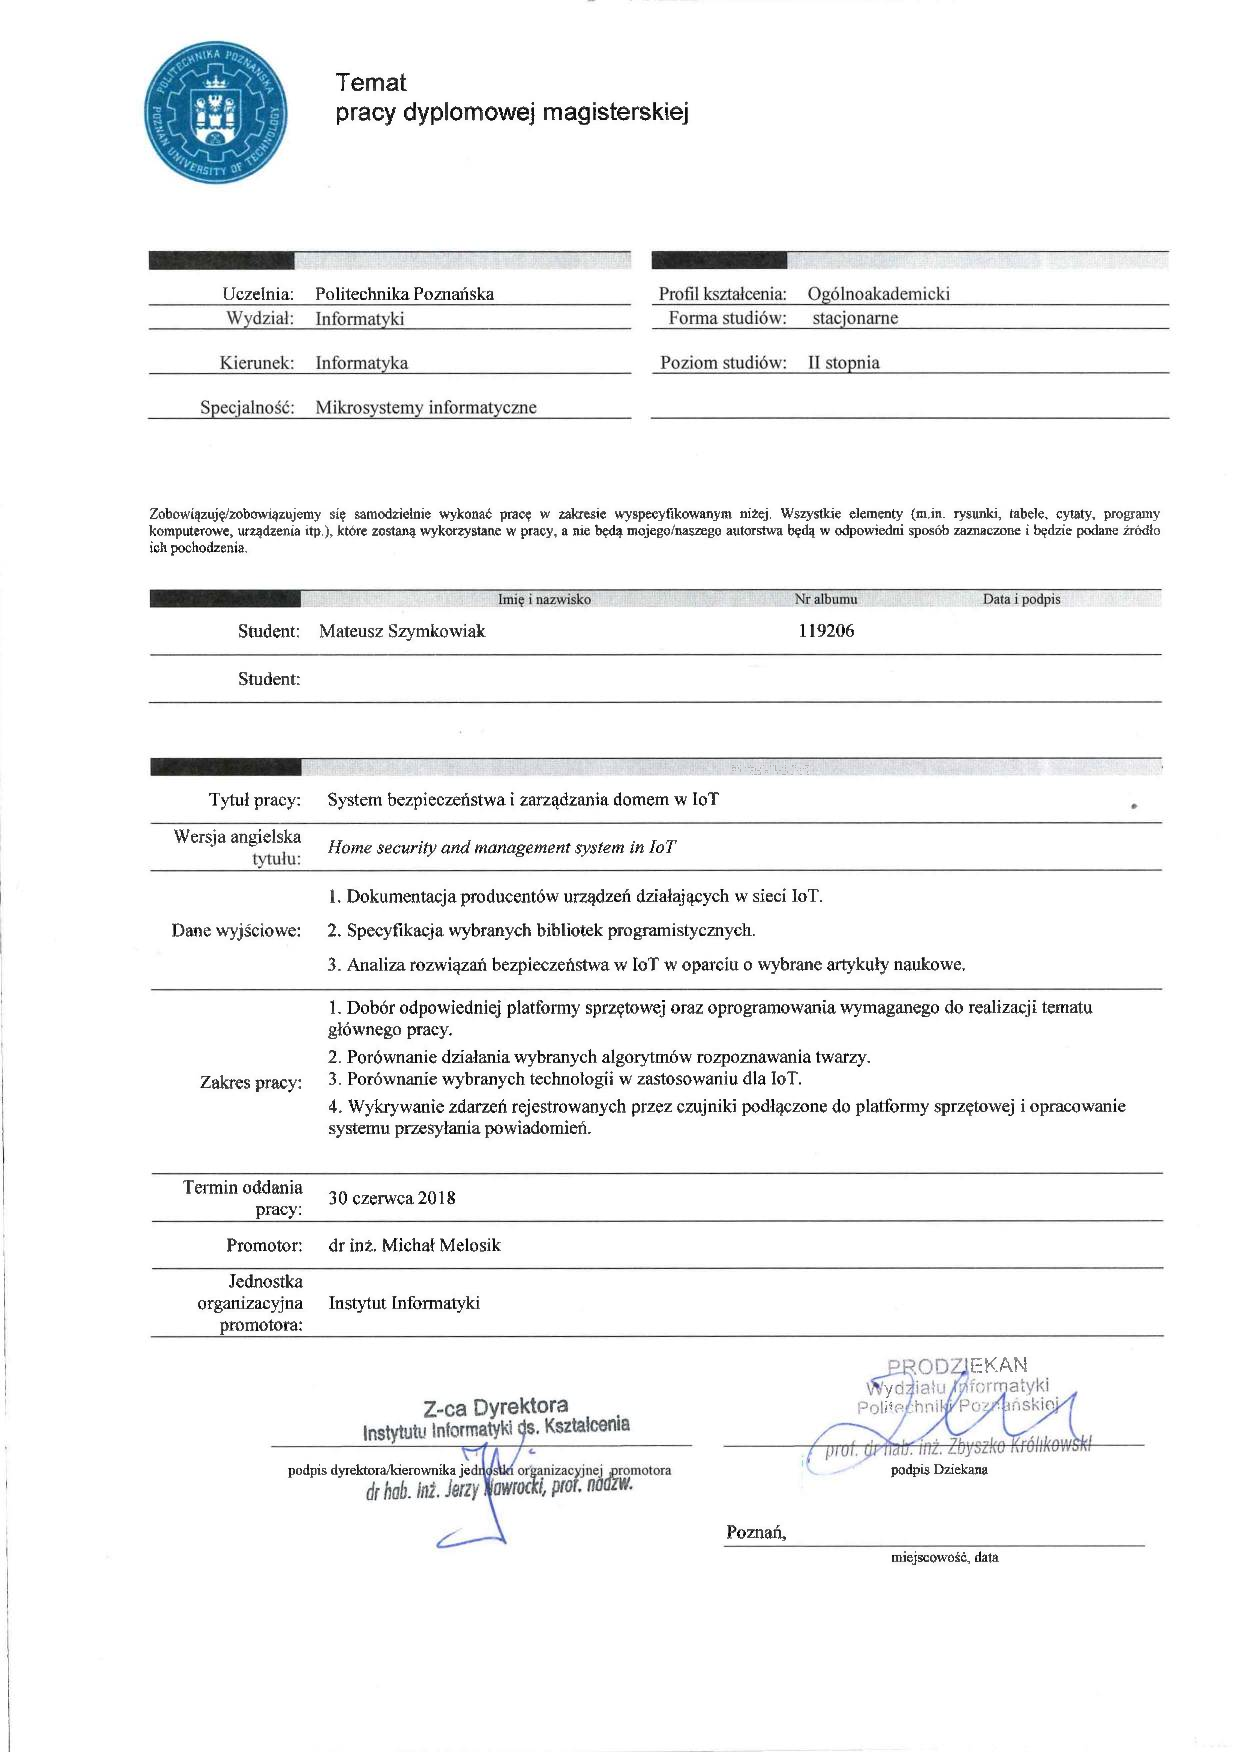
\includepdf[pages={1}]{./pictures/karta_pracy.pdf}

%%%%%%%%%%%%%%%%%%%%%%%%		STRESZCZENIE
\vspace*{\fill}
\begin{center}
{\centering \Huge \bfseries Streszczenie}\\
\end{center}
W pracy zaprezentowano system bezpieczeństwa i zarządzania domem w Internet of Things. Głównymi obiektami badań, na którym skupiono się w tej pracy są systemy detekcji oraz rozpoznawania twarzy. Na potrzeby tej pracy utworzono aplikację internetową umożliwiającą sprawne testowanie wybranych algorytmów, sieci neuronowych oraz usług pozwalających na analizę obrazu. Z powodu niewystarczającej mocy obliczeniowej platformy Raspberry Pi, przetestowano środowiska Azure oraz AWS pozwalające na uruchomienie aplikacji w chmurze.
\\
\\
\\
\begin{center}
 {\Huge \bfseries  Abstract}\\
\end{center}
english
\\
\\
\\
\\
\\
\\
\\
\\
\\
\vspace*{\fill}
%%%%%%%%%%%%%%%%%%%%%%%%		SPIS TREŚCI

\tableofcontents

%%%%%%%%%%%%%%%%%%%%%%%%	WSTĘP
\chapter{Wstęp}
Internet rzeczy (Internet of Things -IoT) to koncepcja przedstawiająca sieć urządzeń fizycznych połączonych inteligentną siecią KNX lub internetową, komunikujących się między sobą i wymieniających dane. Podstawowym celem IoT jest stworzenie inteligentnych przestrzeni- miast, budynków lub systemów związanych z życiem codziennym. Jednym z zastosowań takich systemów są inteligentne domy (smart homes), wykorzystujące czujniki oraz aktuatory do zarządzania domem.

Na potrzeby tej pracy opracowano system bezpieczeństwa oparty o system detekcji i rozpoznawania twarzy na obrazie.

%TODO dodać coś o przetwarzani obrazu, rozpoznawaniu twarzy itd

W rozdziale ,,Cel i zakres pracy'' przedstawiono główne założenia projektu oraz zakres prac autora.

W rozdziale ,,Wstęp teoretyczny'' omówiono podstawowe zagadnienia związane z treścią tej pracy magisterskiej.

W rozdziale ,,Przegląd dostępnych metod rozpoznawania twarzy'' porównano możliwości kilku z dostępnych usług lub oprogramowania pozwalającego na rozpoznawanie twarzy.

W rozdziale ,,System zarządzania metodami rozpoznawania twarzy'' przedstawiono strukturę stworzonej aplikacji, jej podział na moduły oraz wybrane dla każdego z nich środowisko uruchomieniowe.

W rozdziale ,,Aplikacja internetowa'' zaprezentowano wszystkie strony utworzone na potrzeby projektu.

W rozdziale ,,Aplikacja konsolowa'' omówiono sposób wykorzystania wcześniej opisanych usług oraz algorytmy odpowiedzialne za działanie systemu do testowania różnych rozwiązań dla problemu identyfikacji twarzy.

W rozdziale ,,Aplikacja konsolowa do zarządzania domem'' opisano sposób wykorzystania czujników oraz kamery podłączonej bezpośrednio do platformy Raspberry Pi.

W rozdziale ,,Porównanie wykorzystanych technologi'' zbadano oraz porównano skuteczność działania technologi wybranych na potrzeby tej pracy.

W rozdziale ,,Podsumowanie'' zawarto podsumowanie zgromadzonych informacji oraz przedstawiono wnioski wynikające z przeprowadzonych badań.



%TODO dodać opisy kolejnych rozdziałów


%%%%%%%%%%%%%%%%%%%%%%%%	CEL I ZAKRES PRAC
\chapter{Cel i zakres prac}
Celem pracy było stworzenie systemu bezpieczeństwa i zarządzania domem w IoT. Głównymi założeniami było opracowanie systemu pozwalającego na porównanie wybranych metod i usług pozwalających na analizę obrazu oraz kontrolę stanu czujników podłączonych do systemu. IoT jest bardzo prężnie rozwijającą się ideą, dlatego postanowiono porównać wybrane technologie i usługi ułatwiające zarządzanie oraz integrację z takimi aplikacjami.

Jako platformę sprzętową wybrano bardzo popularne w zastosowaniach IoT urządzenie Raspberry Pi 3. Z powodu jego ograniczonych zasobów obliczeniowych zintegrowano chmurowe usługi Azure oraz AWS. Zakres pracy obejmuje następujące zagadnienia:
\begin{itemize}
\item dobór odpowiedniej platformy sprzętowej oraz oprogramowania,
\item porównanie działania wybranych algorytmów detekcji oraz rozpoznawania twarzy,
\item wybór i porównanie wybranych technologi umożliwiających integrację z systemami IoT,
\item wykrywanie zdarzeń rejestrowanych przez wybrane czujniki
%TODO is it really needed?
\item opracowanie systemu przesyłania powiadomień
\item porównanie przydatności zintegrowanych usług w zastosowaniu dla systemu bezpieczeństwa domu
\end{itemize}

%%%%%%%%%%%%%%%%%%%%%%%%	PODSTAWY TEORETYCZNE 
\chapter{System zarządzania domem w IoT}
\begin{figure}[H]
	\centering
	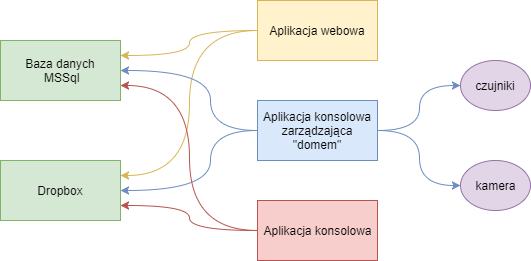
\includegraphics[scale=0.8]{schemat_systemu.png}
	\caption{Budowa systemu zarządzania domem}
	\label{fig:schemat_systemu}
\end{figure}
Aplikację powstałą na potrzeby tej pracy można podzielić na 3 moduły, które zostały przedstawione na rysunku \ref{fig:schemat_systemu}, a składają się na nie :
\begin{itemize}
\item Aplikacja webowa- interfejs pozwalający na zlecanie nowych zadań aplikacji konsolowej oraz odczyt wyników przesłanych przez nią oraz przez program zarządzający domem,
\item Aplikacja konsolowa- przetwarza zadania detekcji oraz rozpoznawania twarzy zlecone za pomocą aplikacji webowej,
\item Program zarządzający domem- przekazuje cyklicznie odczytywane dane z czujników oraz wykryte ruchy do bazy danych, w celu dalszej obróbki przez pozostałe moduły.
\end{itemize}
Na usługi pomocnicze wykorzystane w projekcie składają się
\begin{itemize}
\item baza danych- przechowywanie danych o dodanych zadaniach, wynikach, nauczonych sieciach neuronowych oraz osobach,
\item dropbox- przechowywanie większych plików- obrazów oraz nauczonych modeli sieci.
\end{itemize}

\section{Aplikacja webowa}
Aplikacja webowa jest jedyną częścią systemu, do której użytkownik może mieć bezpośredni dostęp. Strona powstała w celu maksymalnego uproszczenia procesu badania kolejnych algorytmów i usług, które różniły się sposobem podawania danych wejściowych, sposobem uczenia oraz formatem zwracanych odpowiedzi. Do pozostałych zalet takiego rozwiązania należy ułatwienie przechowywania danych, poprzez umieszczenie ich we wspólnym miejscu co pomaga, w późniejszej interpretacji wyników.
\begin{figure}[H]
	\centering
	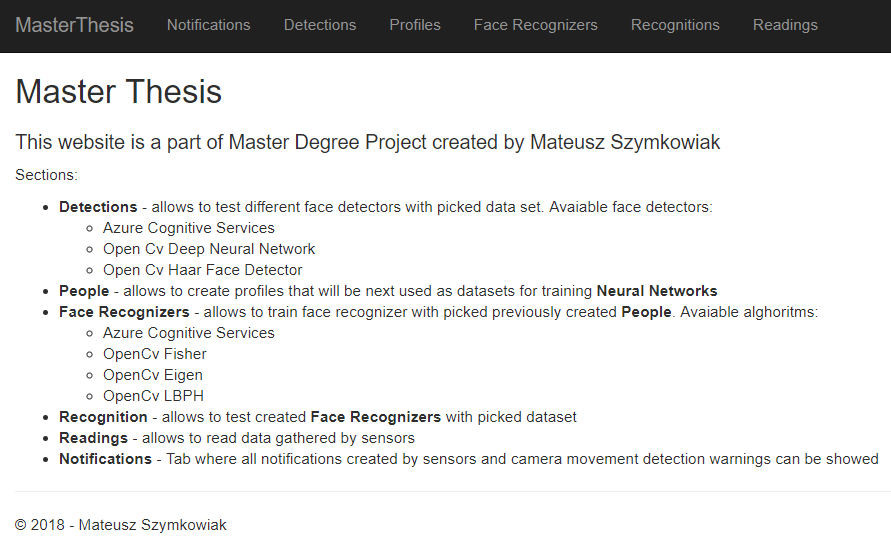
\includegraphics[scale=0.7]{aplikacja_webowa_razor_widok.png}
	\caption{Wygląd strony głównej}
	\label{fig:strona_glowna_razor}
\end{figure}
Zgodnie z interfejsem przedstawionym na rysunku \ref{fig:strona_glowna_razor}, strona została podzielona na 5 głównych sekcji:
\begin{itemize}
\item Detections- detekcje,
\item People- ludzie,
\item Neural Networks- sieci neuronowe,
\item Recognition- rozpoznawanie,
\item Sensor Readings- odczyty sensorów.
\end{itemize}

\subsection{Technologie}
Aplikacja webowa powstała w najnowszej kompilacji .NET Core 2, będącej międzyplatformową strukturą open source o wysokiej wydajności służącą do tworzenia nowoczesnych aplikacji internetowych opartych na usługach chmurowych. Logika biznesowa aplikacji została zaprogramowana w języku C\#. Warstwa widoku powstała w dwóch dostępnych rozwiązaniach, nieznacznie różniących się wyglądem, ale znacznie odbiegających od siebie sposobem działania. Przed omówieniem poszczególnych rozwiązań przedstawiono, krótkie definicje wykorzystanego wzorca projektowego MVC oraz technologii SPA

\subsubsection{Wzorzec projektowy MVC}
\begin{figure}[H]
	\centering
	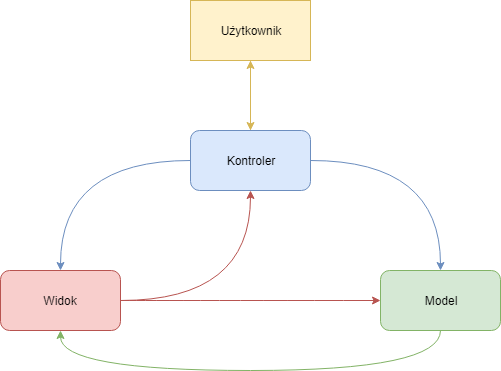
\includegraphics[scale=0.8]{mvc.png}
	\caption{Schemat klasycznego wzorca MVC}
	\label{fig:schemat_mvc}
\end{figure}
Strona internetowa powstała na bazie bardzo popularnego wśród programistów wzorca projektowego MVC. Założenia wzorca Model-Widok-Kontroler są bardzo proste, ich składowymi są:
\begin{itemize}
\item Model- reprezentuje logikę biznesową. Tutaj znajdują się wszelkie obiekty, które służą do wykonywania zaimplementowanej funkcjonalności danej aplikacji,
\item Widok- jest warstwą prezentacji. Odpowiada za prezentację logiki biznesowej (Modelu) użytkownikowi w przystępny sposób,
\item Kontroler- obsługuje żądania użytkownika. Odebrane zadania oddelegowuje do odpowiednich modeli.
\end{itemize}

\subsubsection{Single Page Application}
Single Page Application (SPA) to aplikacja lub strona internetowa, która w całości wczytuje się za jednym razem. Cały potrzebny do działania strony kod (HTML, CSS, JavaScript) przesyłany jest na początku lub dodawany dynamicznie w kawałkach, zwykle w odpowiedzi na interakcje generowane przez użytkownika.
Sposób działania takiej aplikacji jest zbliżony do odczuć towarzyszących korzystaniu z aplikacji desktopowej lub mobilnej. 

\subsubsection{Rozwiązanie 1- Razor Pages}
Pierwsza wersja została oparta o strony tworzone w technologi Razor Pages opartej o składnię Razor oraz podstawowe technologie webowe: HTML i CSS. Taki sposób tworzenia warstwy prezentacji jest zalecany dla aplikacji .NET Core, ponieważ pozwala zminimalizować ilość pracy wymaganej na jej utworzenie oraz zapewnia bardzo prosty proces wdrożenia. Aplikacja utworzona z pomocą Razor'a została zaprezentowana na rysunku \ref{fig:strona_glowna_razor}.

\subsubsection{Rozwiązanie 2- Angular 4}
Druga wersja widoku aplikacji oferuje dostęp do tych samych możliwości co pierwsze rozwiązanie, ale powstała przy pomocy frameworka webowego- Angular 4. Strona główna widoczna jest na rysunku \ref{fig:strona_glowna_angular}. Angular jest open sourcowym frameworkiem używanym do tworzenia aplikacji SPA (Single Page Application), napisany w języku TypeScript i wspierany oraz rozwijany przez Google.
\begin{figure}[H]
	\centering
	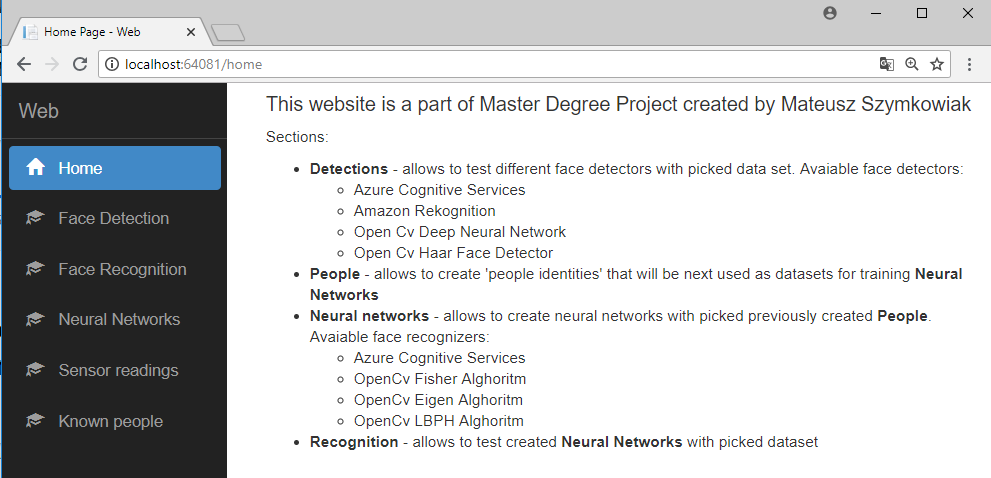
\includegraphics[scale=0.6]{aplikacja_webowa_angular_widok.png}
	\caption{Strona główna widoku utworzonym w Angular 4}
	\label{fig:strona_glowna_angular}
\end{figure}

\subsection{Detections}
Detections jest stroną odpowiedzialną za wykrywanie twarzy na obrazach przesłanych do systemu. Na głównej stronie możemy zobaczyć wszystkie zlecone detekcje, zarówno nowe jak i już zakończone.
\begin{figure}[H]
	\centering
	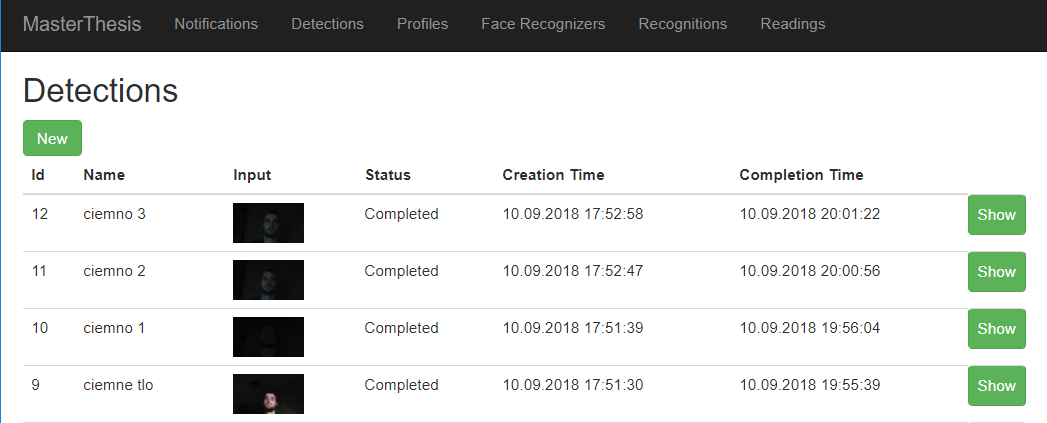
\includegraphics[scale=0.6]{detections.png}
	\caption{Widok detekcji twarzy}
	\label{fig:detections}
\end{figure}
Przycisk 'New' widoczny na \ref{fig:detections} pozwala na stworzenie nowego zadania wykrycia twarzy na obrazie, które zostanie przetworzone przez moduł aplikacji konsolowej. Na formularzu z rysunku \ref{fig:new_detection} należy podać nazwę zadania oraz za pomocą przycisku 'Wybierz plik' wybrać obraz w formacie png,jpg lub jpeg znajdujący się na dysku użytkownika.
\begin{figure}[H]
	\centering
	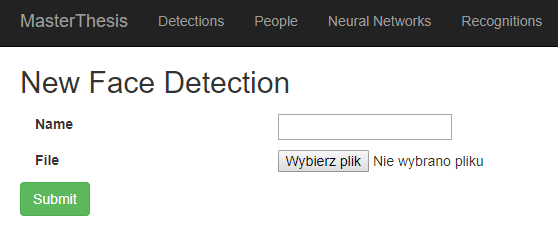
\includegraphics[scale=0.6]{new_detection.png}
	\caption{Tworzenie nowej detekcji}
	\label{fig:new_detection}
\end{figure}
Użycie przycisku 'Show' widocznego przy każdym zadaniu detekcji na rysunku \ref{fig:detections}, pozwoli na wyświetlenie szczegółów związanych z requestem, w tym wyników jeśli zadanie zostało zakończone.
\begin{figure}[H]
	\centering
	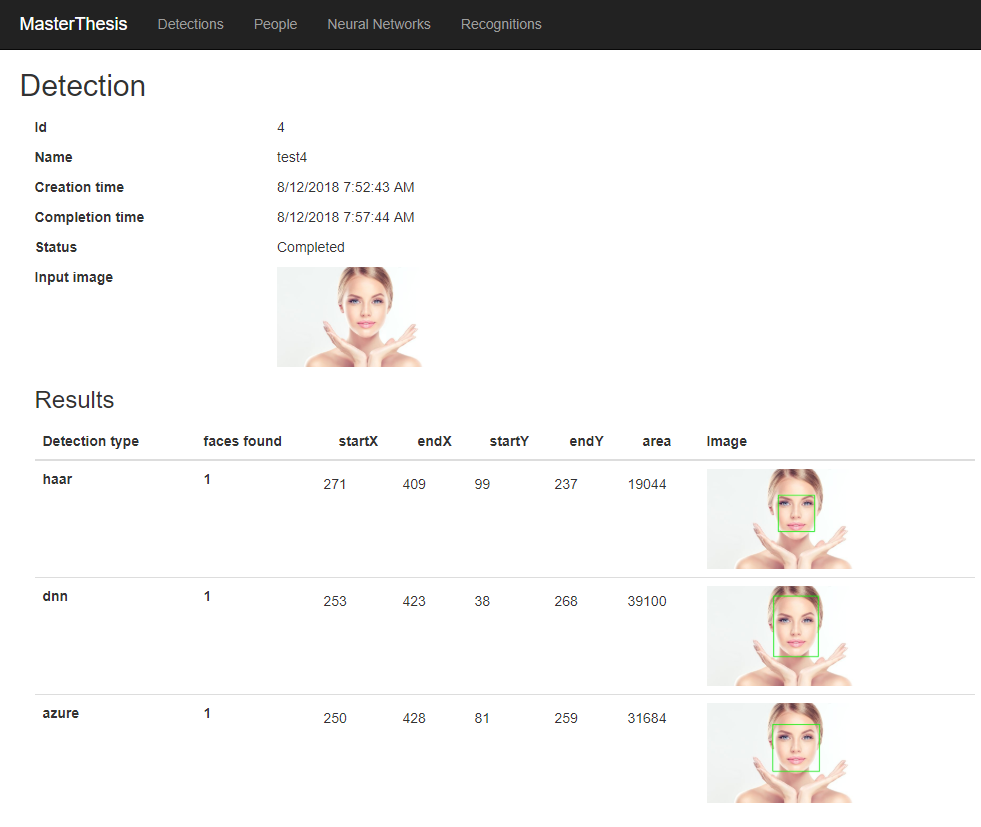
\includegraphics[scale=0.6]{detekcja_z_wynikami.png}
	\caption{Widok zakończonej detekcji}
	\label{fig:detekcja_zakonczona}
\end{figure}
Strona ze zdjęcia \ref{fig:detekcja_zakonczona} pozwala sprawdzić datę utworzenia oraz zakończenia zadania, obraz wejściowy, szczegółowe informacje o obszarze zidentyfikowanym jako twarz oraz sposobie jej wykrycia.
\subsection{People}
Strona 'People' służy do tworzenia nowych znanych tożsamości, które później mogą zostać wykorzystane jako dane uczące podczas trenowania sieci neuronowych. Do każdej osoby musi zostać przypisany zasób minimum 2 zdjęć. W przypadku braku możliwości wykrycia twarzy na zdjęciu, zostanie ono zignorowane podczas procesu nauczania.
\begin{figure}[H]
	\centering
	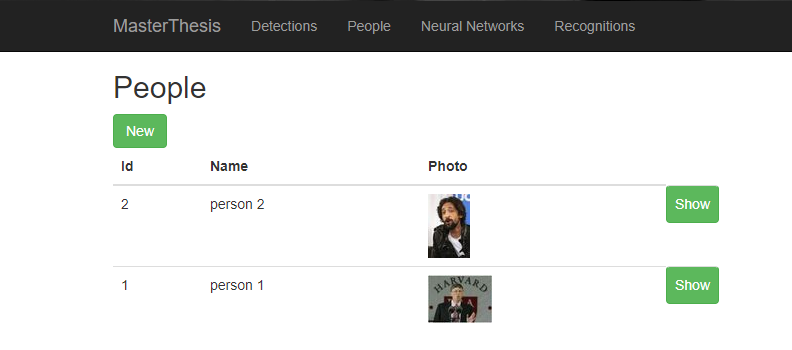
\includegraphics[scale=0.6]{people.png}
	\caption{Lista utworzonych ludzi}
	\label{fig:people}
\end{figure}
Nowa osoba może zostać utworzona w podobny sposób jak request detekcji twarzy. Jedyną różnicą jest wymóg wyboru kilku obrazów.
\begin{figure}[H]
	\centering
	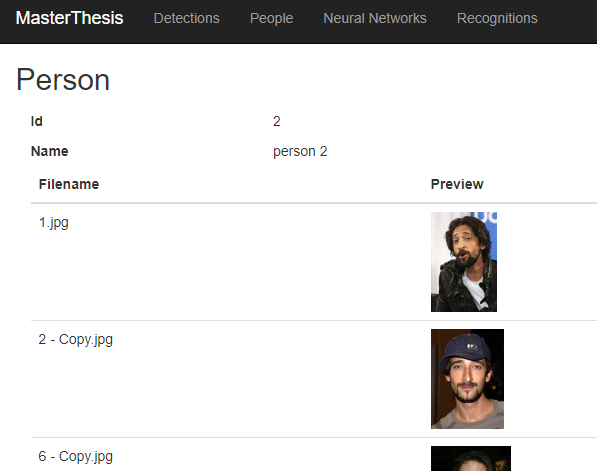
\includegraphics[scale=0.6]{person.png}
	\caption{Widok osoby}
	\label{fig:person}
\end{figure}
Utworzona osoba nie może być modyfikowana. Pierwsze załadowanie widoku osoby może trwać wydłużony czas z powodu procesu generowania linków do plików magazynowanych w usłudze Dropbox.

\subsection{Neural Networks}
\begin{figure}[H]
	\centering
	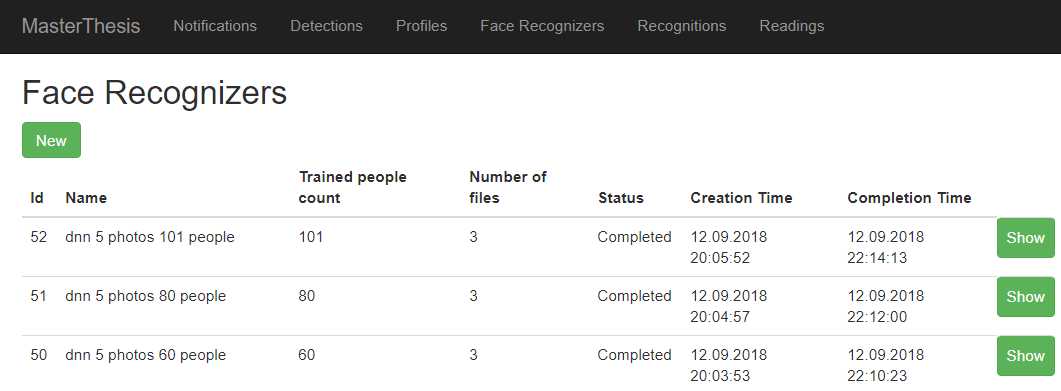
\includegraphics[scale=0.6]{neural_networks.png}
	\caption{Strona przedstawiająca istniejące grupy usług rozpoznawania tożsamości}
	\label{fig:sieci_neuronowe}
\end{figure}
W zakładce 'Neural Networks' użytkownik ma możliwość stworzenia grupy wybranych usług i sieci neuronowych, które zostaną nauczone rozpoznawać tożsamości utworzone w zakładce 'People'.
\begin{figure}[H]
	\centering
	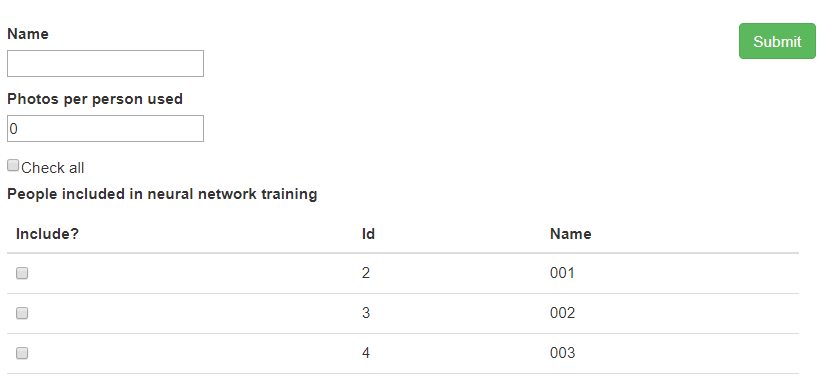
\includegraphics[scale=0.6]{nowa_siec.png}
	\caption{Tworzenie nowej grupy sieci neuronowych}
	\label{fig:nowa_siec}
\end{figure}
Każda istniejąca osoba zostanie wyświetlona jako checkbox, który należy zaznaczyć jeśli użytkownik chce by dana osoba została wykorzystana podczas procesu trenowania. Należy wybrać minimum 2 osoby, w przypadku wyboru mniejszej ilości osób, użytkownik zostanie poinformowany o tej konieczności.

Widok ukazany na rysunku \ref{fig:sieci_neuronowe} pozwala sprawdzić ile osób zostało użytych w procesie nauki oraz ile sieci neuronowych zostało utworzonych. Wyświetlenie jednej z grup pozwoli na uzyskanie bardziej szczegółowych informacji na temat wykorzystanych osób i utworzonych sieci, patrz rysunek \ref{fig:siec_neuronowa}.
\begin{figure}[H]
	\centering
	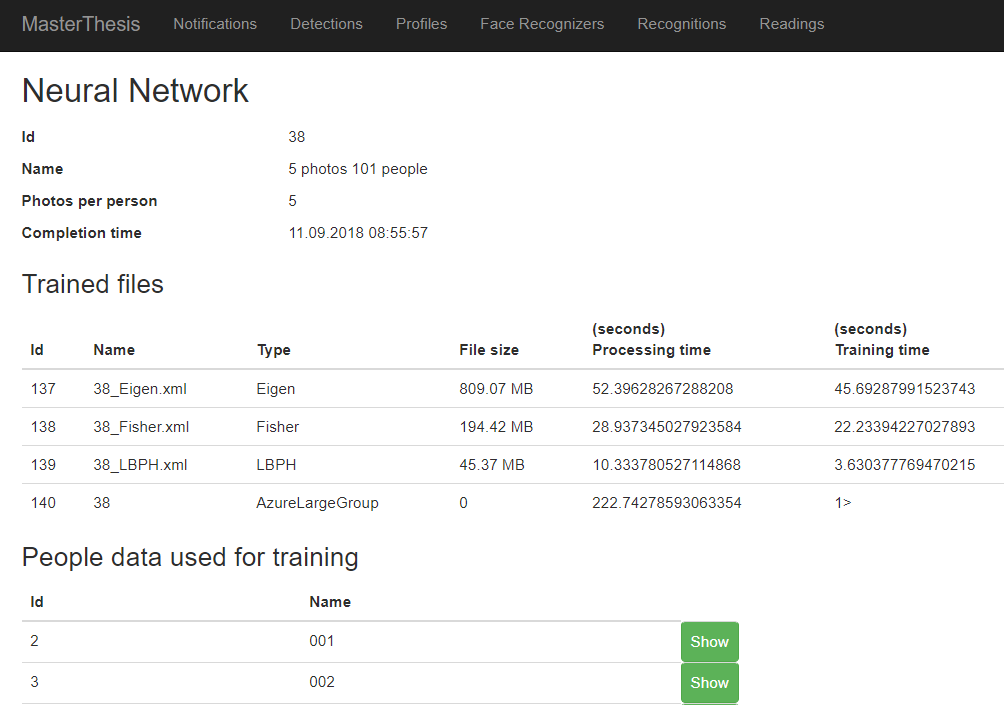
\includegraphics[scale=0.6]{siec_neuronowa.png}
	\caption{Szczegółowe informacje o grupie sieci neuronowych}
	\label{fig:siec_neuronowa}
\end{figure}

\subsection{Recognitions}
W sekcji 'Recognitions' użytkownik ma możliwość wykorzystać wcześniej utworzone zbiory sieci neuronowych w celu identyfikacji tożsamości na zdjęciu przedstawiającym pojedynczą osobę.
\begin{figure}[H]
	\centering
	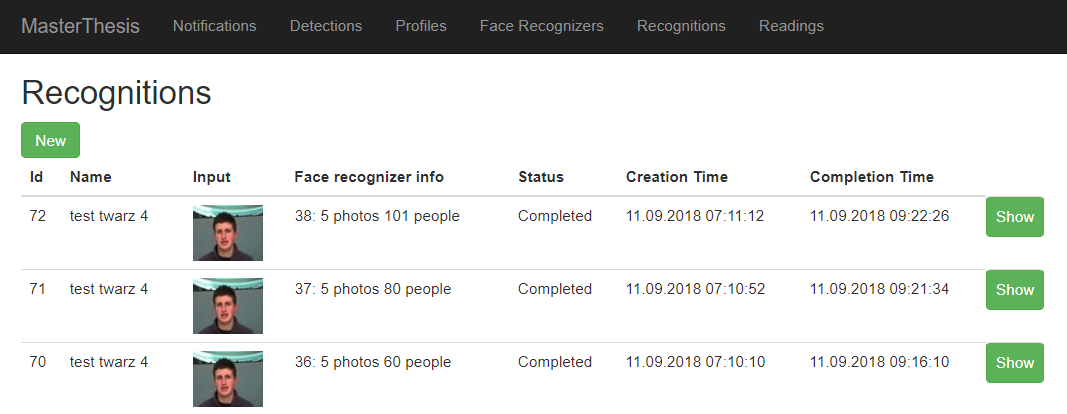
\includegraphics[scale=0.6]{recognitions.png}
	\caption{Lista zadań identyfikacji osoby}
	\label{fig:recognitions}
\end{figure}
Podobnie jak na pozostałych stronach, podczas tworzenia nowego zadania użytkownik będzie musiał uzupełnić prosty formularz. W formularzu przedstawionym na rysunku \ref{fig:new_recognition} należy załączyć jedno zdjęcie oraz wybrać grupę sieci neuronowych, która ma zostać wykorzystana do identyfikacji tożsamości osoby.
\begin{figure}[H]
	\centering
	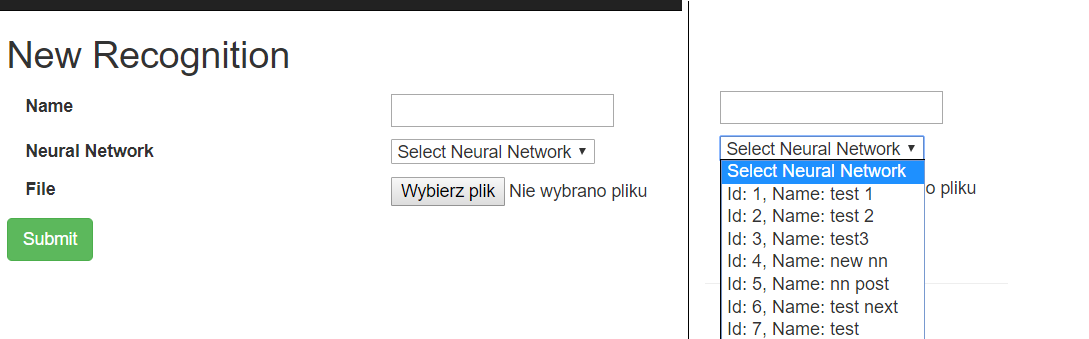
\includegraphics[scale=0.6]{new_recognition.png}
	\caption{Formularz tworzenia zadania identyfikacji}
	\label{fig:new_recognition}
\end{figure}
Po zakończonym procesie identyfikacji opisanym w kolejnym podrozdziale, użytkownik może wyświetlić wynik uzyskany przez każdą sieć dostępną w grupie. Przykładowy rezultat widoczny jest na zdjęciu \ref{fig:recognition}.
\begin{figure}[H]
	\centering
	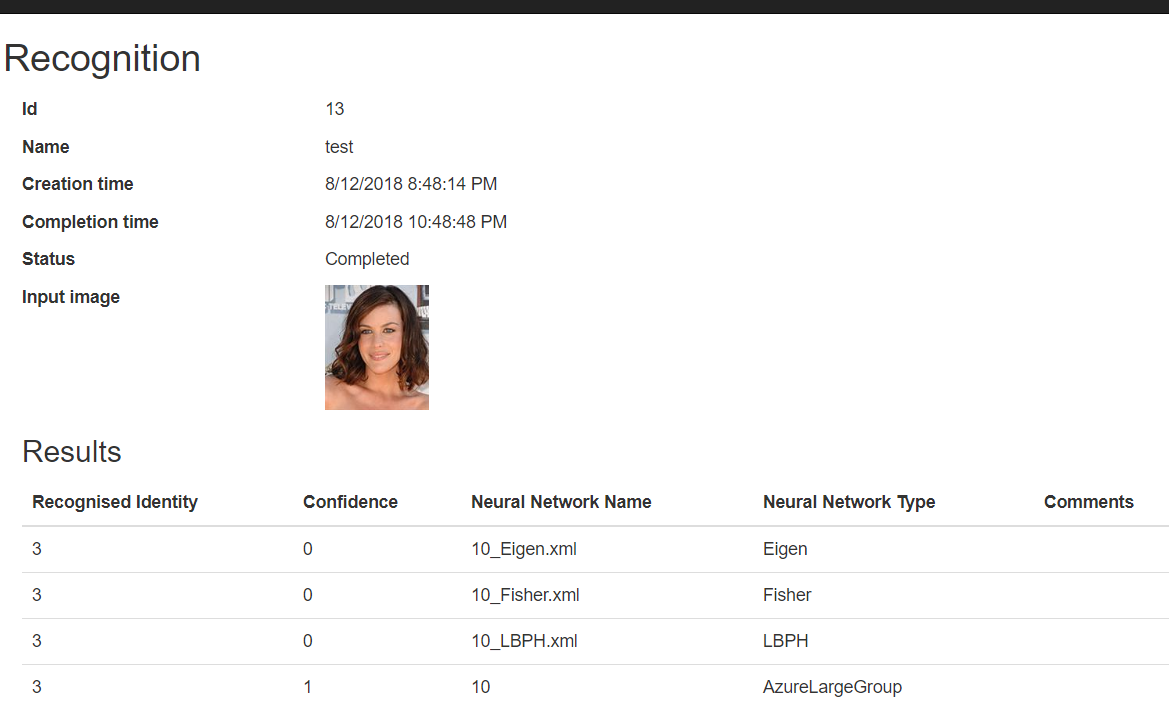
\includegraphics[scale=0.6]{recognition.png}
	\caption{Zakończony request identyfikacji}
	\label{fig:recognition}
\end{figure}

\section{Aplikacja konsolowa}
Aplikacja konsolowa powstała w celu przetwarzania czasochłonnych zadań w tle, tak by użytkownik aplikacji webowej nie doświadczał długich czasów ładowania oraz ewentualnych błędów podczas przerwania sesji lub połączenia internetowego ze stroną. Aplikacja konsolowa uruchamiana jest co 5 minut i przetwarza zadania trzech typów w kolejności widocznej na rysunku \ref{fig:worker_proces}. Poszczególne procesy zostały szerzej opisane w kolejnych podrozdziałach.
\begin{figure}[H]
	\centering
	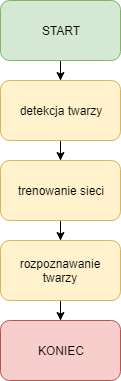
\includegraphics[scale=0.6]{worker_proces.png}
	\caption{Proces działania aplikacji konsolowej}
	\label{fig:worker_proces}
\end{figure}



\subsection{Technologie}


\subsection{Proces wykrywania twarzy}
Uogólniony proces detekcji twarzy na obrazie został przedstawiony na grafie \ref{fig:wykrywanie_proces}. Szczegółowy proces dla każdej z metod detekcji przedstawiono w rozdziale \ref{detekcja_twarzy}.
\begin{figure}[H]
	\centering
	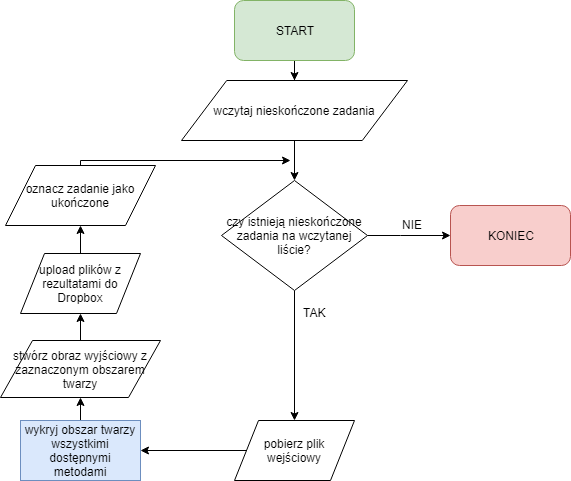
\includegraphics[scale=0.6]{wykrywanie_twarzy.png}
	\caption{Proces wykrywania twarzy}
	\label{fig:wykrywanie_proces}
\end{figure}

\subsection{Proces trenowania sieci neuronowych}
Proces trenowania sieci został przedstawiony na grafie \ref{fig:trenowanie_proces}, szczegółowe informacje o przygotowaniu danych uczących i procesie nauczania zostały opisane w kolejnej sekcji.
\begin{figure}[H]
	\centering
	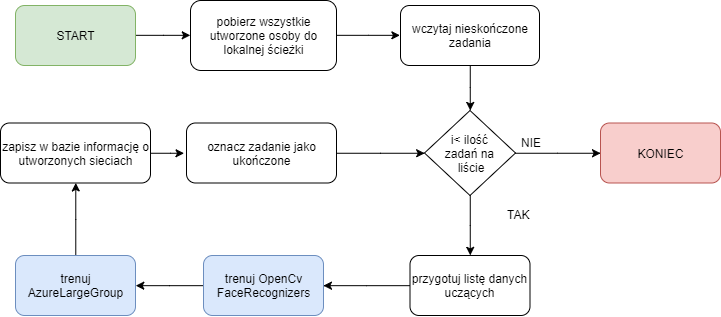
\includegraphics[scale=0.6]{proces_nauczania.png}
	\caption{Proces trenowania sieci}
	\label{fig:trenowanie_proces}
\end{figure}

\subsubsection{Przygotowanie danych trenujących} \label{przygotowanie_danych_uczących}

\subsubsection{Trenowanie sieci} \label{trenowanie_sieci}

\subsection{Proces rozpoznawania twarzy}


\section{Program zarządzający domem}

%%%%%%%%%%%%%%%%%%%%%%%%	System detekcji twarzy
\chapter{System detekcji twarzy} \label{detekcja_twarzy}
\section{Przegląd dostępnych systemów}
\section{OpenCv}
\subsection{Haar}
\subsection{Dnn}
\section{Azure Cognitive Services}

%\begin{figure}[H]
	\centering
	\includegraphics[scale=0.58]{schemat_dzialania.png}
	\caption{System pomiarowo-wykonawczy}
\end{figure}
System opisany w tym raporcie został oparty o trzy podstawowe urządzenia:
\begin{itemize}
\item urządzenie mobilne z oprogramowaniem Android,
\item Arduino Uno,
\item ogniwo Peltiera.
\end{itemize}
Za pomocą telefonu lub tabletu z modułem Bluetooth, użytkownik łączy się z system regulacji temperatury zbudowanym wokół Arduino. Aplikacja pozwala na wybór opcji związanych z regulacją, które zostają przesłane do Arduino za pomocą, komunikacji Bluetooth. Płytka Arduino interpretuje odczytane dane, następnie dokonuje pomiaru temperatury oraz oblicza sygnał sterujący PWM, za pomocą, którego zostaje wysterowane ogniwo Peltiera.

Podstawowe informacje na temat każdego z elementów przedstawiono w kolejnych sekcjach. Dokładny sposób działania wszystkich składowych opisano w poświęconych im rozdziałach.



\section{Ogniwo Peltiera} %%jest OK
Ogniwo Peltiera jest półprzewodnikowym elementem termoelektrycznym, wykorzystującym zjawisko Peltiera do przekazywania ciepła, dzięki czemu może pełnić funkcje grzejące i chłodzące.
\subsection{Efekt Peltiera} %%jest OK
Efekt Peltiera to zjawisko termoelektryczne polegające na bezpośrednim oddziaływaniu różnicy napięć na temperaturę oraz różnicy temperatury na pojawienie się napięcia. Efekt Peltiera opisuje zjawisko pojawienia się 
obiektu grzejącego i chłodzącego podczas zasilenia połączonych ze sobą różnych rodzajów przewodników, półprzewodników. Jego nazwa pochodzi od francuskiego naukowca. Zjawisko zaobserwowano po utworzeniu obwody z dwóch różnych przewodów, miedzianego i bizmutowego, które zostało następnie zasilone. Jeden z drutów nagrzewał się, a drugi ochładzał. Zimny pręt został umieszczony w odizolowanym obiekcie, w wyniku czego powstała lodówka o niskiej wydajności.

Kolejne eksperymenty Peltiera potwierdziły, że różne metale i półprzewodniki podłączone do zasilanego obwodu uzyskują właściwości przyjmowania lub oddawania energii cieplnej, co skutkuje ochładzaniem się elementu przyjmującego ciepło oraz ogrzewaniem materiału, który oddaje energię przyjętą przez element pochłaniający. Badania wykazały, że ilość przekazywanej w procesie energii, zależy od materiałów, z których wykonano części, natężenia przepływającego prądu oraz czasu jaki przepływał przez obwód. Na różnicę temperatur bezpośredni wpływ ma różnica zdolności termoelektrycznych miedzy materiałami oraz wartość natężenia prądu.

W określonej jednostce czasu, ilość pochłanianego i wydzielanego ciepła można opisać następującym wzorem:

\begin{equation}
	\Delta Q / \Delta T= \Pi _{AB} I
\end{equation}
\begin{math}
	\Pi _{AB} 
\end{math} 
-współczynnik Peltiera obwodu,	\\
\begin{math}
	\Delta Q
\end{math} 
-ciepło,	\\
\begin{math}
	\Delta T
\end{math}  
-czas,	\\
\begin{math}
	I
\end{math} 
-prąd.\\

W wyniku odwrócenia kierunku przepływu prądu przez układ, dochodzi do odwrócenia właściwości pochłaniania i oddawania energii materiałów.
Odkryte przez Peltiera właściwości pozwoliły na powstanie półprzewodnikowego modułu termoelektrycznego wykorzystanego w tej pracy, nazywanego ogniwem Peltiera. Odkrycie to zapoczątkowało późniejsze powstanie lodówek turystycznych, w których wykorzystuje się ogniwo Peltiera. Znajduje ono zastosowanie również w chłodnictwie przemysłowym i laboratoryjnym.

\subsection{Budowa ogniwa} %%jest OK
Ogniwo Peltiera zbudowane jest z dwóch równolegle położonych płytek ceramicznych, pomiędzy którymi rozłożone są naprzemiennie przewodniki typu ,,n'' oraz ,,p''. 
\begin{figure}[H]
	\centering
	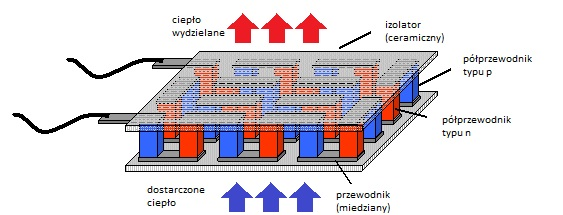
\includegraphics[scale=0.8]{budowaPeltier.jpg}
	\caption{Budowa modułu Peltiera}
\end{figure}
Półprzewodnikami wykorzystanymi do budowy ogniwa są tellurk oraz bizmut, które połączono ze sobą miedzianymi blaszkami. Istotą działania modułów Peltiera są zachodzące zmiany temperatur na połączeniach półprzewodników n-p, p-n, w wyniku przepływu prądu elektrycznego, którego wartość ma wpływ na ilość ciepła, które może zostać przetransportowana między stronami. Półprzewodnik typu n charakteryzuje się nadmiarową ilością elektronów, a typu p ich niewystarczalną ilością do wejścia na wyższy poziom energetyczny. Podczas przepływu prądu, elektrony przemieszczają się między poziomami energetycznymi, co w zależności od typu półprzewodnika oznacza zapotrzebowanie na dostarczenie energii (strona zimna) lub powoduje jej wydzielanie (strona ciepła). Niestety moduł nie jest idealny i część energii zostaje utracona w wyniku czego dochodzi również do ogrzania komponentów ogniwa.

Przydatną cechą modułów Peltiera jest możliwość połączenia ich kaskadowo tak by strona ciepła kolejnego ogniwa stykała się ze stroną zimną poprzedniego, co może pozwolić na wzrost wydajności układu. Ze względu na dużą ilość wydzielanego ciepła, zaleca się wykorzystanie pasty termoprzewodzącej oraz radiatorów po stronie ciepłej ogniwa.



\section{Arduino} %%jest OK
Arduino to sprzęt komputerowy i oprogramowanie stworzone przez firmę o tej samej nazwie, skupiające się na tworzenie zestawów uruchomieniowych opartych o mikrokontrolery z rodziny ATmega. Układ umieszczany jest na pojedynczej płytce drukowanej, z wyprowadzonymi wejściami i wyjściami układu. Język programowania  również nazywa się Arduino i został oparty o język C i C++. Najpopularniejszym ich produktem jest Arduino Uno. Wszystkie produkty wydawane są z otwartą licencją sprzętową i oprogramowania, dlatego na to na rynku dostępne są liczne klony płytek, zgodne z jej oryginalną specyfikacją. Urządzenia Arduino
może zostać wykorzystane jako samodzielny obiekt lub może być podłączone do komputera użytkownika.
\subsection{Hardware}%%jest OK
\begin{figure}[H]
	\centering
	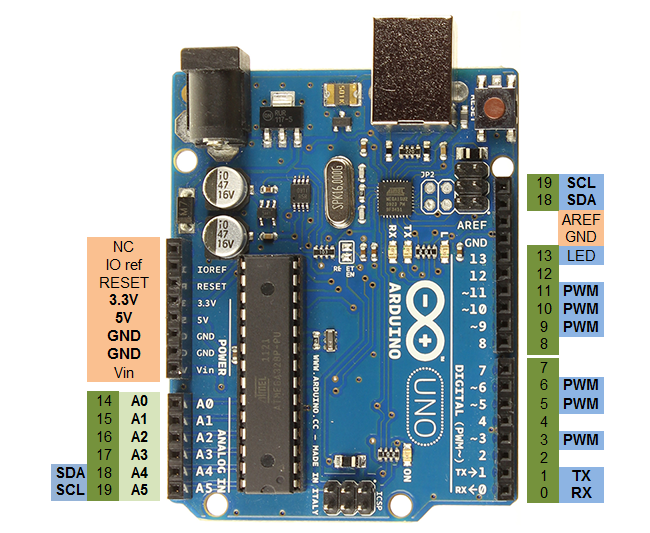
\includegraphics[scale=0.4]{ArduinoUno_pinout.png}
	\caption{Rozmieszczenie pinów dostępnych w Arduino Uno}
\end{figure}
Typowa płytka Arduino składa sie z mikrokontrolera, cyfrowych wejść/wyjść oraz wejść analogowych. Poza tym można na niej znaleźć takie interfejsy jak UART oraz USB do połączenia z komputerem, SPI i I2C do komunikacji z urządzeniami elektronicznymi.

W tej pracy wykorzystano płytkę Arduino Uno. Arduino Uno oparte jest o 8-bitowy mikrokontroler ATmega328, który uzupełniono elementami pozwalającymi na łatwiejsze programowanie wykorzystując port RS232 oraz sterowanie wyjściami mikrokontrolera. Płytka zawiera 5V regulator napięcia oraz rezonator kwarcowy o częstotliwości oscylacji 16MHz. Wyjścia mikrokontrolera zostały opisane i wyprowadzone jako żeńskie piny na obrzeżach płytki. Zastosowane rozwiązanie pozwala na łatwe podpięcie modułów rozszerzających funkcjonalność Arduino, nazywanych \textit{shieldami}. 

Arduino Uno posiada 6 wejść analogowych, 14 cyfrowych pinów wejścia/wyjścia, gdzie aż 6 z nich może zostać wykorzystane do generowania sygnału PWM. Oprócz tego można na niej znaleźć wyprowadzenia zasilania 3.3V i 5V. Piny analogowe zostały oznaczone literką A.
\newpage
\subsection{Programowanie}%%jest OK
\begin{figure}[H]
	\centering
	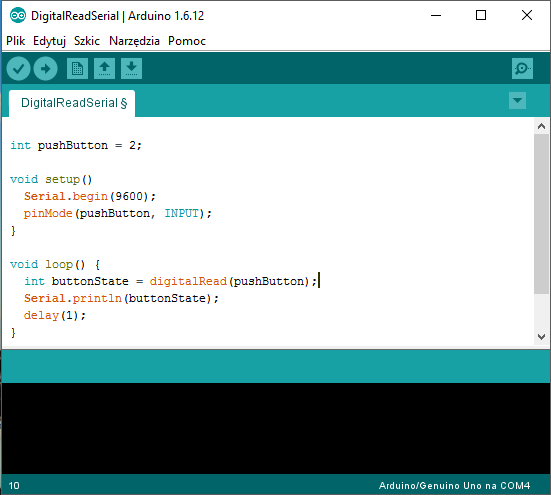
\includegraphics[scale=0.8]{pictures/arduinoIDE.PNG}
	\caption{Arduino IDE- przykładowy program}
	\label{ArduinoPodstawoweFunkcje}
\end{figure}
Do programowania płytek Arduino wykorzystuje się dedykowane oprogramowania Arduino IDE, które powstało na podstawie projektu Wiring oraz interfejs szeregowy RS232. Proces ten został ułatwiony poprzez wcześniejsze zaprogramowanie mikrokontrolera programem rozruchowym, zwalniającym z potrzeby używania zewnętrznego programatora. Oprogramowanie zawiera tak przydatne funkcje jak: kolorowanie składni kodu, automatyczne formatowanie, kompilację oraz wgrywanie programu na urządzenie docelowe. Zaletą Arduino IDE są dostępne opcje monitorowania portu szeregowego komputera w formie tekstowej, wykorzystując narzędzie ,,Monitor portu szeregowe'' oraz w postaci wykresu używając ,,Kreślarki''. Zawarta w programie biblioteka Wiring, będąca biblioteką C/C++, pozwala na ułatwienie wykonywania podstawowych operacji wejścia/wyjścia.

Aby stworzyć działający projekt należy zdefiniować dwie podstawowe funkcje:
\begin{itemize}
\item setup()- funkcja wykonywana tylko raz, wywoływana na początku programu w celu załadowania ustawień,
\item loop()- główne ciało programu, funkcja wykonywana jest wielokrotnie przez cały czas działania programu.
\end{itemize}


\section{Technologie internetowe}
\subsection{Cordova} %%jest OK
Apache Cordova to popularny framework służący do tworzenia aplikacji mobilnych w językach znanych deweloperom webowym. Cordova pozwala na utworzenie aplikacji na urządzenia mobilne wykorzystując HTML5, CSS3 oraz JavaScript. Jest to ciekawe rozwiązanie pozwalające na uniezależnienie się od środowisk programistycznych, specyficznych dla danej platformy jak np. Android Studio dla urządzeń z oprogramowaniem Android.

Cordova pozwala na napisanie jednej aplikacji, która następnie zostanie odpowiednio przetworzona, tak by działała na odpowiedniej platformie dystrybucji- urządzeniu Android lub iOS. W ten sposób uzyskuje się aplikację hybrydową, która nie jest w pełni natywna ze względu na interfejs użytkownika, który jest generowany w powłoce przeglądarki oraz nie w pełni webowa, bo zostaje skompilowana w paczkę dystrybucyjną, np. o rozszerzeniu app. Aplikacja ma dostęp do podzespołów telefonu, między innymi Bluetooth, WiFi, akcelerometr, GPS. 

\subsection{Ionic Framework}%%jest OK
Ionic to framework służący do tworzenia hybrydowych aplikacji mobilnych wykorzystujących HTML5, CSS i JavaScript. Został zbudowany z wykorzystaniem AngularJS oraz Apache Cordova. Takie rozwiązanie pozwala na dystrybucję aplikacji na różne platformy. Ionic mozna określić jako paczkę narzędzi, usług i stylów odpowiadającą za kreowanie przyjaznego interfejsu użytkownika. Jest ona odpowiednikiem wzbogaconego Bootstrapa w wersji dla aplikacji mobilnych.

Ionic zapewnia wszystkie funkcje dostępne w podstawowych SDK (zestaw narzędzi dla programistów, niezbędny w tworzeniu aplikacji na dany system) dla danej platformy. Interakcja z niestandardowymi komponentami i metodami udostępnionymi przez Ionic, możliwa jest poprzez wykorzystanie języka AngularJS.

\subsection{HTML}%%jest OK
HTML (HyperText Markup Language) to hipertekstowy język znaczników służący do tworzenia stron i aplikacji internetowych. W tej pracy wykorzystano HTML 5, który wywodzi się z języka HTML 4 i XHTML 1. Został on przyjęty za aktualny standard i jest wspierany przez wszystkie środowiska i producentów przeglądarek internetowych. Wraz z kaskadowymi arkuszami stylów i JavaScriptem tworzy on grupę najpopularniejszych technologii internetowych. HTML opisuje strukturę strony w sposób semantyczny, nadając treści dokumentu odpowiednie właściwości i funkcje, takie jak formowanie hiperłącza, list, nagłówków i akapitów. Do pozostałych funkcji tego języka należy możliwość załączania plików, plików graficznych i innych multimediów. Uzupełnieniem HTML jest CSS, który został opisany w kolejnym punkcie.

\subsection{Kaskadowe arkusze stylów}%%jest OK
Kaskadowe arkusze stylów (z ang. Cascading Style Sheets, w skrócie CSS) to język arkuszy stylów służący  do opisywania sposobu prezentacji zawartości dokumentu HTML, stron www. 
Arkusz stylów pozwala na opisanie wszystkich elementów dokumentu internetowego, takich jak: czcionka, kolor i rozmiar czcionki, interlinie, skalowanie elementów w zależności od rozmiarów otwartego okna oraz pozycjonowanie ich.

CSS został stworzony przez organizację W3C w 1996 roku w celu rozdzielenia warstwy prezentacji od warstwy danych. Uzyskane rozwiązanie pozwoliło na zwiększenie przejrzystości dokumentów HTML oraz ograniczyło ilość zmian wymaganych do wprowadzania podczas zmieniania stylu, który został wykorzystany na licznych podstronach.

\subsection{JavaScript}%%jest OK
JavaScript to dynamiczny, skryptowy język programowania wysokiego poziomu. Należy do grupy trzech najważniejszych języków, których musi się nauczyć każdy deweloper serwisów internetowych. Jest obsługiwany przez wszystkie nowoczesne przeglądarki internetowe bez potrzeby instalowania dodatkowych wtyczek. Mimo dużego podobieństwa w nazwie, języki Java i JavaScript znacznie różnią się składnią i dostępnymi bibliotekami. Język ten był wzorowany na C i przejął po nim między innymi funkcje warunkowe i pętle. W odróżnieniu od C jest to język prawie w pełni obiektowy.

Głównym zadaniem JavaScriptu jest zapewnienie interaktywności interfejsu użytkownika, czyli reakcja na wydarzenia takie jak wciśnięcie przycisku, wyświetlanie okien dialogowych, wywoływanie cyklicznych funkcji oraz aktualizowanie danych wyświetlanych na stronie. Poza tym pozwala na tworzenie ciasteczek i pobieranie informacji o przeglądarce użytkownika. JavaScript ma ograniczony dostęp do zasobów komputera użytkownika.

Do rozszerzenia funkcjonalności JavaScriptu wykorzystuje się lekkie biblioteki programistyczne takie jak jQuery, AngularJS ułatwiające manipulację obiektowym modelem dokumentu (z ang.DOM- Document Object Model), wykonywanie zapytań AJAX oraz dodawanie animacji na wyświetlanej stronie.

Skrypt JavaScript może zostać umieszczony na końcu dokumentu HTML, którego dotyczy, jednak ze względu na czytelność kodu i wymagany dostęp do niego dla wszystkich podstron, najczęściej zostaje umieszczony w osobnym pliku dodanym do projektu.

\subsection{AngularJS}%%jest OK
AngularJS to oparty na JavaScripcie, utworzony na otwartej licencji framework do tworzenia aplikacji internetowych, którego deweloperem jest Google. Głównym celem frameworka jest ułatwienie procesu deweloperskiego i testowania aplikacji poprzez wprowadzenie MVC (kontroler modelu widoku) po stronie użytkownika oraz MVVM (z ang. Model--viev--view-Model) w celu rozdzielenia kodu interfejsu od części logicznej.

AngularJS zaczyna pracę od przeszukania strony HTML w poszukiwaniu niestandardowych znaczników, które interpretuje i przypisuje do wejścia/wyjścia zmiennych wykorzystanych w JavaScipcie. Framework dopasowuje się do dokumentu HTML i rozszerza jego funkcjonalność o możliwość dynamicznego wyświetlania danych i aktualizowania widoku aplikacji, dzięki zaimplementowanemu dwukierunkowemu połączeniu między modelem i widokiem. Takie rozwiązanie pozwala znacznie ograniczyć ilość wymaganych do wykonania operacji w DOM.

Struktura programu w AngularJS składa się między innymi na zadeklarowany moduł aplikacji, kontroler i serwis.
\lstset{language=Java}
\begin{lstlisting} 
var app = angular.module('myApp', []);
app.controller('myController', function($scope) {
    $scope.firstName = "John";
    $scope.lastName = "Doe";
    $scope.personAge=myService.getAge();
})
app.service('myService', function() {
	var age=15;
    this.getAge = function () {
        return age;
    }
});
\end{lstlisting}
Zadaniem kontrolerów jest ingerowanie w interfejs użytkownika, reagowanie na wciśnięcia guzików oraz dokonywania zmian w wyświetlanych informacjach. \textit{Scope} to obiekt łączący ze sobą dane modelu i widoku. Serwisy tworzy się w celu zapewnienia funkcjonalności nie wpływającej bezpośrednio na interfejs, takiej jak np. pobieranie danych otrzymanych przez moduł Bluetooth, a następnie udostępnienie ich kontrolerowi poprzez funkcje zwracające wybrane dane.


\section{Komunikacja}
\subsection{Bluetooth}%%jest OK
Bluetooth to standard bezprzewodowej technologii wymiany danych na krótkim dystansie, pomiędzy urządzeniami typu klawiatura, komputer, bezprzewodowy głośnik, urządzenie mobilne, a w tym przypadku również Arduino. Został wymyślony przez firmę Ericsson w 1994 roku i został uznany za bezprzewodową alternatywę dla popularnego interfejsu RS232. Specyfikacja standardu Bluetooth obejmuje trzy klasy mocy nadawczej, 1-3 o zasięgu odpowiednio 100m, 10m i 1 metra w otwartej przestrzeni. W tej pracy wykorzystano moduł klasy 2, o zasięgu do 10 metrów.

Bluetooth pracuje na częstotliwości od 2402 do 2480 MHz, która jest globalnym standardem pasma częstotliwości krótkiego zasięgu dla zastosowań przemysłowych, naukowych i medycznych. Bluetooth dzieli wymieniane dane na pakiety. Każdy z nich zostaje wysłany na jeden z 79 wyznaczonych kanałów Bluetooth, których przepustowość wynosi 1 MHz. W przypadku modułów Bluetooth Low Energy o niższym poborze energii, kanałów jest jedynie 40, bo odstępy między nimi wynoszą aż 2 MHz. Protokół ten został oparty na strukturze Master-Slave. Zainicjować połączenie miedzy modułami może jedynie Master (w tym przypadku urządzenie mobilne), a Slave (moduł Bluetooth podłączony do Arduino) jedynie je zaakceptować. W tym protokole nie występuje problem z synchronizowaniem danych, dlatego że połączone ze sobą urządzenia otrzymują wspólny zegar, do którego działania zostaje dopasowany proces wysyłania i odbierania danych.

\subsection{UART}%%jest OK
UART ( z ang. Universal Asynchronous Receiver and Transmitter) to interfejs komunikacji szeregowej, szeroko wykorzystywany do przesyłania i odbierania danych asynchronicznie. Asynchroniczność oznacza, że dane są wysyłane nieregularnie. Ich początek i koniec jest oznaczony specjalnym symbolem. Interfejs UART został wykorzystany w tym projekcie do komunikacji między Arduino i modułem Bluetooth.
Procesor ATmega 328 znajdujący się na płytce Arduino Uno posiada specjalnie wyprowadzone piny portu szeregowego:
\begin{itemize}
\item{RXD- wejście szeregowe (,,Receive Data''),}
\item{TXD- wyjście szeregowe (,,Transmit Data'').}
\end{itemize}
Zaletą interfejsu UART jest posiadany przez niego bufor danych przeznaczony do tymczasowego przechowywania informacji w sytuacji, gdy są one szybko transmitowane.
Ten rodzaj transmisji danych charakteryzuje się również tym, że nadajnik i odbiornik nie posiada wspólnego sygnału zegarowego. W tym przypadku każde z urządzeń działa w takt własnego zegara. Podczas połączenia urządzeń należy pamiętać, aby oba miały ustawioną taką samą częstotliwość taktowania zegara.

\subsection{1-Wire}%%jest OK
One Wire to systemowa magistrala komunikacji elektronicznej pomiędzy urządzeniami, zapewniająca przesyłanie danych oraz zasilanie urządzenia przez pojedynczy kabel. Proces ten jest możliwy dzięki stopniowemu ładowaniu kondensatora znajdującego się w odbiorniku, a następnie wykorzystanie zgromadzonej energii do zasilenia urządzenia. Do magistrali może zostać podłączonych wiele urządzeń. Każdemu z nich przydzielany jest indywidualny adres 64-bitowy. Komunikację z urządzeniami inicjuje master, w tym przypadku mikrokontroler.

Przedstawiony protokół jest bardzo podobny do I2C, ale ze względu na wykorzystanie jedynie jednej linii danych, charakteryzuje się niższą prędkością przesyłania. Układ zazwyczaj zasilany jest napięciem o wartości 5V i służy do komunikacji pomiędzy niewielkimi urządzeniami, takimi jak np. termometr cyfrowy i mikrokontroler.



%%%%%%%%%%%%%%%%%%%%%%%%	System rozpoznawania twarzy
\chapter{System rozpoznawania twarzy} \label{rozpoznawanie_twarzy}
\section{Przegląd dostępnych systemów}
\section{OpenCv}
\subsection{Fisher}
\subsection{LBPH}
\subsection{Eigen}
\section{Azure Cognitive Services}
%\begin{figure}[H]
	\centering
	\includegraphics[scale=0.58]{schemat_dzialania.png}
	\caption{System pomiarowo-wykonawczy}
\end{figure}
System opisany w tym raporcie został oparty o trzy podstawowe urządzenia:
\begin{itemize}
\item urządzenie mobilne z oprogramowaniem Android,
\item Arduino Uno,
\item ogniwo Peltiera.
\end{itemize}
Za pomocą telefonu lub tabletu z modułem Bluetooth, użytkownik łączy się z system regulacji temperatury zbudowanym wokół Arduino. Aplikacja pozwala na wybór opcji związanych z regulacją, które zostają przesłane do Arduino za pomocą, komunikacji Bluetooth. Płytka Arduino interpretuje odczytane dane, następnie dokonuje pomiaru temperatury oraz oblicza sygnał sterujący PWM, za pomocą, którego zostaje wysterowane ogniwo Peltiera.

Podstawowe informacje na temat każdego z elementów przedstawiono w kolejnych sekcjach. Dokładny sposób działania wszystkich składowych opisano w poświęconych im rozdziałach.



\section{Ogniwo Peltiera} %%jest OK
Ogniwo Peltiera jest półprzewodnikowym elementem termoelektrycznym, wykorzystującym zjawisko Peltiera do przekazywania ciepła, dzięki czemu może pełnić funkcje grzejące i chłodzące.
\subsection{Efekt Peltiera} %%jest OK
Efekt Peltiera to zjawisko termoelektryczne polegające na bezpośrednim oddziaływaniu różnicy napięć na temperaturę oraz różnicy temperatury na pojawienie się napięcia. Efekt Peltiera opisuje zjawisko pojawienia się 
obiektu grzejącego i chłodzącego podczas zasilenia połączonych ze sobą różnych rodzajów przewodników, półprzewodników. Jego nazwa pochodzi od francuskiego naukowca. Zjawisko zaobserwowano po utworzeniu obwody z dwóch różnych przewodów, miedzianego i bizmutowego, które zostało następnie zasilone. Jeden z drutów nagrzewał się, a drugi ochładzał. Zimny pręt został umieszczony w odizolowanym obiekcie, w wyniku czego powstała lodówka o niskiej wydajności.

Kolejne eksperymenty Peltiera potwierdziły, że różne metale i półprzewodniki podłączone do zasilanego obwodu uzyskują właściwości przyjmowania lub oddawania energii cieplnej, co skutkuje ochładzaniem się elementu przyjmującego ciepło oraz ogrzewaniem materiału, który oddaje energię przyjętą przez element pochłaniający. Badania wykazały, że ilość przekazywanej w procesie energii, zależy od materiałów, z których wykonano części, natężenia przepływającego prądu oraz czasu jaki przepływał przez obwód. Na różnicę temperatur bezpośredni wpływ ma różnica zdolności termoelektrycznych miedzy materiałami oraz wartość natężenia prądu.

W określonej jednostce czasu, ilość pochłanianego i wydzielanego ciepła można opisać następującym wzorem:

\begin{equation}
	\Delta Q / \Delta T= \Pi _{AB} I
\end{equation}
\begin{math}
	\Pi _{AB} 
\end{math} 
-współczynnik Peltiera obwodu,	\\
\begin{math}
	\Delta Q
\end{math} 
-ciepło,	\\
\begin{math}
	\Delta T
\end{math}  
-czas,	\\
\begin{math}
	I
\end{math} 
-prąd.\\

W wyniku odwrócenia kierunku przepływu prądu przez układ, dochodzi do odwrócenia właściwości pochłaniania i oddawania energii materiałów.
Odkryte przez Peltiera właściwości pozwoliły na powstanie półprzewodnikowego modułu termoelektrycznego wykorzystanego w tej pracy, nazywanego ogniwem Peltiera. Odkrycie to zapoczątkowało późniejsze powstanie lodówek turystycznych, w których wykorzystuje się ogniwo Peltiera. Znajduje ono zastosowanie również w chłodnictwie przemysłowym i laboratoryjnym.

\subsection{Budowa ogniwa} %%jest OK
Ogniwo Peltiera zbudowane jest z dwóch równolegle położonych płytek ceramicznych, pomiędzy którymi rozłożone są naprzemiennie przewodniki typu ,,n'' oraz ,,p''. 
\begin{figure}[H]
	\centering
	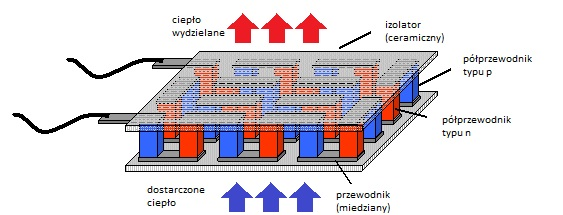
\includegraphics[scale=0.8]{budowaPeltier.jpg}
	\caption{Budowa modułu Peltiera}
\end{figure}
Półprzewodnikami wykorzystanymi do budowy ogniwa są tellurk oraz bizmut, które połączono ze sobą miedzianymi blaszkami. Istotą działania modułów Peltiera są zachodzące zmiany temperatur na połączeniach półprzewodników n-p, p-n, w wyniku przepływu prądu elektrycznego, którego wartość ma wpływ na ilość ciepła, które może zostać przetransportowana między stronami. Półprzewodnik typu n charakteryzuje się nadmiarową ilością elektronów, a typu p ich niewystarczalną ilością do wejścia na wyższy poziom energetyczny. Podczas przepływu prądu, elektrony przemieszczają się między poziomami energetycznymi, co w zależności od typu półprzewodnika oznacza zapotrzebowanie na dostarczenie energii (strona zimna) lub powoduje jej wydzielanie (strona ciepła). Niestety moduł nie jest idealny i część energii zostaje utracona w wyniku czego dochodzi również do ogrzania komponentów ogniwa.

Przydatną cechą modułów Peltiera jest możliwość połączenia ich kaskadowo tak by strona ciepła kolejnego ogniwa stykała się ze stroną zimną poprzedniego, co może pozwolić na wzrost wydajności układu. Ze względu na dużą ilość wydzielanego ciepła, zaleca się wykorzystanie pasty termoprzewodzącej oraz radiatorów po stronie ciepłej ogniwa.



\section{Arduino} %%jest OK
Arduino to sprzęt komputerowy i oprogramowanie stworzone przez firmę o tej samej nazwie, skupiające się na tworzenie zestawów uruchomieniowych opartych o mikrokontrolery z rodziny ATmega. Układ umieszczany jest na pojedynczej płytce drukowanej, z wyprowadzonymi wejściami i wyjściami układu. Język programowania  również nazywa się Arduino i został oparty o język C i C++. Najpopularniejszym ich produktem jest Arduino Uno. Wszystkie produkty wydawane są z otwartą licencją sprzętową i oprogramowania, dlatego na to na rynku dostępne są liczne klony płytek, zgodne z jej oryginalną specyfikacją. Urządzenia Arduino
może zostać wykorzystane jako samodzielny obiekt lub może być podłączone do komputera użytkownika.
\subsection{Hardware}%%jest OK
\begin{figure}[H]
	\centering
	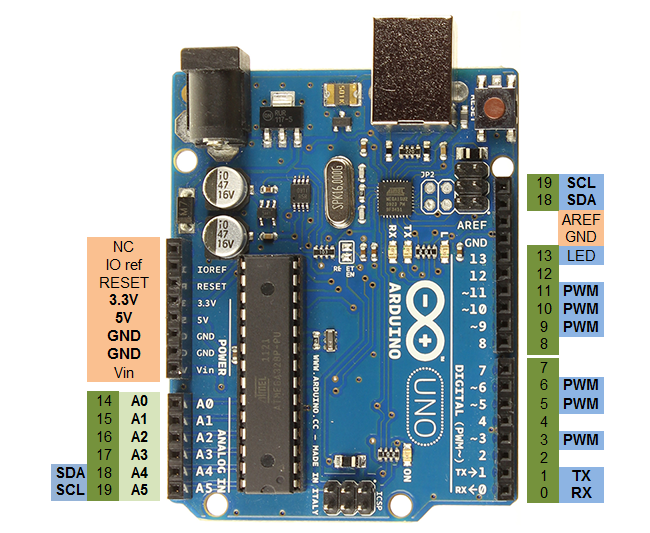
\includegraphics[scale=0.4]{ArduinoUno_pinout.png}
	\caption{Rozmieszczenie pinów dostępnych w Arduino Uno}
\end{figure}
Typowa płytka Arduino składa sie z mikrokontrolera, cyfrowych wejść/wyjść oraz wejść analogowych. Poza tym można na niej znaleźć takie interfejsy jak UART oraz USB do połączenia z komputerem, SPI i I2C do komunikacji z urządzeniami elektronicznymi.

W tej pracy wykorzystano płytkę Arduino Uno. Arduino Uno oparte jest o 8-bitowy mikrokontroler ATmega328, który uzupełniono elementami pozwalającymi na łatwiejsze programowanie wykorzystując port RS232 oraz sterowanie wyjściami mikrokontrolera. Płytka zawiera 5V regulator napięcia oraz rezonator kwarcowy o częstotliwości oscylacji 16MHz. Wyjścia mikrokontrolera zostały opisane i wyprowadzone jako żeńskie piny na obrzeżach płytki. Zastosowane rozwiązanie pozwala na łatwe podpięcie modułów rozszerzających funkcjonalność Arduino, nazywanych \textit{shieldami}. 

Arduino Uno posiada 6 wejść analogowych, 14 cyfrowych pinów wejścia/wyjścia, gdzie aż 6 z nich może zostać wykorzystane do generowania sygnału PWM. Oprócz tego można na niej znaleźć wyprowadzenia zasilania 3.3V i 5V. Piny analogowe zostały oznaczone literką A.
\newpage
\subsection{Programowanie}%%jest OK
\begin{figure}[H]
	\centering
	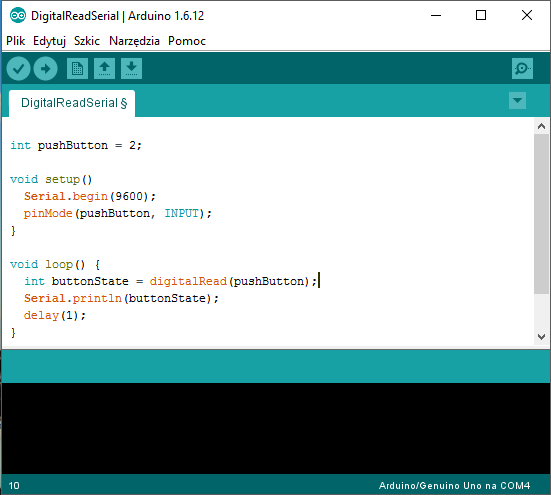
\includegraphics[scale=0.8]{pictures/arduinoIDE.PNG}
	\caption{Arduino IDE- przykładowy program}
	\label{ArduinoPodstawoweFunkcje}
\end{figure}
Do programowania płytek Arduino wykorzystuje się dedykowane oprogramowania Arduino IDE, które powstało na podstawie projektu Wiring oraz interfejs szeregowy RS232. Proces ten został ułatwiony poprzez wcześniejsze zaprogramowanie mikrokontrolera programem rozruchowym, zwalniającym z potrzeby używania zewnętrznego programatora. Oprogramowanie zawiera tak przydatne funkcje jak: kolorowanie składni kodu, automatyczne formatowanie, kompilację oraz wgrywanie programu na urządzenie docelowe. Zaletą Arduino IDE są dostępne opcje monitorowania portu szeregowego komputera w formie tekstowej, wykorzystując narzędzie ,,Monitor portu szeregowe'' oraz w postaci wykresu używając ,,Kreślarki''. Zawarta w programie biblioteka Wiring, będąca biblioteką C/C++, pozwala na ułatwienie wykonywania podstawowych operacji wejścia/wyjścia.

Aby stworzyć działający projekt należy zdefiniować dwie podstawowe funkcje:
\begin{itemize}
\item setup()- funkcja wykonywana tylko raz, wywoływana na początku programu w celu załadowania ustawień,
\item loop()- główne ciało programu, funkcja wykonywana jest wielokrotnie przez cały czas działania programu.
\end{itemize}


\section{Technologie internetowe}
\subsection{Cordova} %%jest OK
Apache Cordova to popularny framework służący do tworzenia aplikacji mobilnych w językach znanych deweloperom webowym. Cordova pozwala na utworzenie aplikacji na urządzenia mobilne wykorzystując HTML5, CSS3 oraz JavaScript. Jest to ciekawe rozwiązanie pozwalające na uniezależnienie się od środowisk programistycznych, specyficznych dla danej platformy jak np. Android Studio dla urządzeń z oprogramowaniem Android.

Cordova pozwala na napisanie jednej aplikacji, która następnie zostanie odpowiednio przetworzona, tak by działała na odpowiedniej platformie dystrybucji- urządzeniu Android lub iOS. W ten sposób uzyskuje się aplikację hybrydową, która nie jest w pełni natywna ze względu na interfejs użytkownika, który jest generowany w powłoce przeglądarki oraz nie w pełni webowa, bo zostaje skompilowana w paczkę dystrybucyjną, np. o rozszerzeniu app. Aplikacja ma dostęp do podzespołów telefonu, między innymi Bluetooth, WiFi, akcelerometr, GPS. 

\subsection{Ionic Framework}%%jest OK
Ionic to framework służący do tworzenia hybrydowych aplikacji mobilnych wykorzystujących HTML5, CSS i JavaScript. Został zbudowany z wykorzystaniem AngularJS oraz Apache Cordova. Takie rozwiązanie pozwala na dystrybucję aplikacji na różne platformy. Ionic mozna określić jako paczkę narzędzi, usług i stylów odpowiadającą za kreowanie przyjaznego interfejsu użytkownika. Jest ona odpowiednikiem wzbogaconego Bootstrapa w wersji dla aplikacji mobilnych.

Ionic zapewnia wszystkie funkcje dostępne w podstawowych SDK (zestaw narzędzi dla programistów, niezbędny w tworzeniu aplikacji na dany system) dla danej platformy. Interakcja z niestandardowymi komponentami i metodami udostępnionymi przez Ionic, możliwa jest poprzez wykorzystanie języka AngularJS.

\subsection{HTML}%%jest OK
HTML (HyperText Markup Language) to hipertekstowy język znaczników służący do tworzenia stron i aplikacji internetowych. W tej pracy wykorzystano HTML 5, który wywodzi się z języka HTML 4 i XHTML 1. Został on przyjęty za aktualny standard i jest wspierany przez wszystkie środowiska i producentów przeglądarek internetowych. Wraz z kaskadowymi arkuszami stylów i JavaScriptem tworzy on grupę najpopularniejszych technologii internetowych. HTML opisuje strukturę strony w sposób semantyczny, nadając treści dokumentu odpowiednie właściwości i funkcje, takie jak formowanie hiperłącza, list, nagłówków i akapitów. Do pozostałych funkcji tego języka należy możliwość załączania plików, plików graficznych i innych multimediów. Uzupełnieniem HTML jest CSS, który został opisany w kolejnym punkcie.

\subsection{Kaskadowe arkusze stylów}%%jest OK
Kaskadowe arkusze stylów (z ang. Cascading Style Sheets, w skrócie CSS) to język arkuszy stylów służący  do opisywania sposobu prezentacji zawartości dokumentu HTML, stron www. 
Arkusz stylów pozwala na opisanie wszystkich elementów dokumentu internetowego, takich jak: czcionka, kolor i rozmiar czcionki, interlinie, skalowanie elementów w zależności od rozmiarów otwartego okna oraz pozycjonowanie ich.

CSS został stworzony przez organizację W3C w 1996 roku w celu rozdzielenia warstwy prezentacji od warstwy danych. Uzyskane rozwiązanie pozwoliło na zwiększenie przejrzystości dokumentów HTML oraz ograniczyło ilość zmian wymaganych do wprowadzania podczas zmieniania stylu, który został wykorzystany na licznych podstronach.

\subsection{JavaScript}%%jest OK
JavaScript to dynamiczny, skryptowy język programowania wysokiego poziomu. Należy do grupy trzech najważniejszych języków, których musi się nauczyć każdy deweloper serwisów internetowych. Jest obsługiwany przez wszystkie nowoczesne przeglądarki internetowe bez potrzeby instalowania dodatkowych wtyczek. Mimo dużego podobieństwa w nazwie, języki Java i JavaScript znacznie różnią się składnią i dostępnymi bibliotekami. Język ten był wzorowany na C i przejął po nim między innymi funkcje warunkowe i pętle. W odróżnieniu od C jest to język prawie w pełni obiektowy.

Głównym zadaniem JavaScriptu jest zapewnienie interaktywności interfejsu użytkownika, czyli reakcja na wydarzenia takie jak wciśnięcie przycisku, wyświetlanie okien dialogowych, wywoływanie cyklicznych funkcji oraz aktualizowanie danych wyświetlanych na stronie. Poza tym pozwala na tworzenie ciasteczek i pobieranie informacji o przeglądarce użytkownika. JavaScript ma ograniczony dostęp do zasobów komputera użytkownika.

Do rozszerzenia funkcjonalności JavaScriptu wykorzystuje się lekkie biblioteki programistyczne takie jak jQuery, AngularJS ułatwiające manipulację obiektowym modelem dokumentu (z ang.DOM- Document Object Model), wykonywanie zapytań AJAX oraz dodawanie animacji na wyświetlanej stronie.

Skrypt JavaScript może zostać umieszczony na końcu dokumentu HTML, którego dotyczy, jednak ze względu na czytelność kodu i wymagany dostęp do niego dla wszystkich podstron, najczęściej zostaje umieszczony w osobnym pliku dodanym do projektu.

\subsection{AngularJS}%%jest OK
AngularJS to oparty na JavaScripcie, utworzony na otwartej licencji framework do tworzenia aplikacji internetowych, którego deweloperem jest Google. Głównym celem frameworka jest ułatwienie procesu deweloperskiego i testowania aplikacji poprzez wprowadzenie MVC (kontroler modelu widoku) po stronie użytkownika oraz MVVM (z ang. Model--viev--view-Model) w celu rozdzielenia kodu interfejsu od części logicznej.

AngularJS zaczyna pracę od przeszukania strony HTML w poszukiwaniu niestandardowych znaczników, które interpretuje i przypisuje do wejścia/wyjścia zmiennych wykorzystanych w JavaScipcie. Framework dopasowuje się do dokumentu HTML i rozszerza jego funkcjonalność o możliwość dynamicznego wyświetlania danych i aktualizowania widoku aplikacji, dzięki zaimplementowanemu dwukierunkowemu połączeniu między modelem i widokiem. Takie rozwiązanie pozwala znacznie ograniczyć ilość wymaganych do wykonania operacji w DOM.

Struktura programu w AngularJS składa się między innymi na zadeklarowany moduł aplikacji, kontroler i serwis.
\lstset{language=Java}
\begin{lstlisting} 
var app = angular.module('myApp', []);
app.controller('myController', function($scope) {
    $scope.firstName = "John";
    $scope.lastName = "Doe";
    $scope.personAge=myService.getAge();
})
app.service('myService', function() {
	var age=15;
    this.getAge = function () {
        return age;
    }
});
\end{lstlisting}
Zadaniem kontrolerów jest ingerowanie w interfejs użytkownika, reagowanie na wciśnięcia guzików oraz dokonywania zmian w wyświetlanych informacjach. \textit{Scope} to obiekt łączący ze sobą dane modelu i widoku. Serwisy tworzy się w celu zapewnienia funkcjonalności nie wpływającej bezpośrednio na interfejs, takiej jak np. pobieranie danych otrzymanych przez moduł Bluetooth, a następnie udostępnienie ich kontrolerowi poprzez funkcje zwracające wybrane dane.


\section{Komunikacja}
\subsection{Bluetooth}%%jest OK
Bluetooth to standard bezprzewodowej technologii wymiany danych na krótkim dystansie, pomiędzy urządzeniami typu klawiatura, komputer, bezprzewodowy głośnik, urządzenie mobilne, a w tym przypadku również Arduino. Został wymyślony przez firmę Ericsson w 1994 roku i został uznany za bezprzewodową alternatywę dla popularnego interfejsu RS232. Specyfikacja standardu Bluetooth obejmuje trzy klasy mocy nadawczej, 1-3 o zasięgu odpowiednio 100m, 10m i 1 metra w otwartej przestrzeni. W tej pracy wykorzystano moduł klasy 2, o zasięgu do 10 metrów.

Bluetooth pracuje na częstotliwości od 2402 do 2480 MHz, która jest globalnym standardem pasma częstotliwości krótkiego zasięgu dla zastosowań przemysłowych, naukowych i medycznych. Bluetooth dzieli wymieniane dane na pakiety. Każdy z nich zostaje wysłany na jeden z 79 wyznaczonych kanałów Bluetooth, których przepustowość wynosi 1 MHz. W przypadku modułów Bluetooth Low Energy o niższym poborze energii, kanałów jest jedynie 40, bo odstępy między nimi wynoszą aż 2 MHz. Protokół ten został oparty na strukturze Master-Slave. Zainicjować połączenie miedzy modułami może jedynie Master (w tym przypadku urządzenie mobilne), a Slave (moduł Bluetooth podłączony do Arduino) jedynie je zaakceptować. W tym protokole nie występuje problem z synchronizowaniem danych, dlatego że połączone ze sobą urządzenia otrzymują wspólny zegar, do którego działania zostaje dopasowany proces wysyłania i odbierania danych.

\subsection{UART}%%jest OK
UART ( z ang. Universal Asynchronous Receiver and Transmitter) to interfejs komunikacji szeregowej, szeroko wykorzystywany do przesyłania i odbierania danych asynchronicznie. Asynchroniczność oznacza, że dane są wysyłane nieregularnie. Ich początek i koniec jest oznaczony specjalnym symbolem. Interfejs UART został wykorzystany w tym projekcie do komunikacji między Arduino i modułem Bluetooth.
Procesor ATmega 328 znajdujący się na płytce Arduino Uno posiada specjalnie wyprowadzone piny portu szeregowego:
\begin{itemize}
\item{RXD- wejście szeregowe (,,Receive Data''),}
\item{TXD- wyjście szeregowe (,,Transmit Data'').}
\end{itemize}
Zaletą interfejsu UART jest posiadany przez niego bufor danych przeznaczony do tymczasowego przechowywania informacji w sytuacji, gdy są one szybko transmitowane.
Ten rodzaj transmisji danych charakteryzuje się również tym, że nadajnik i odbiornik nie posiada wspólnego sygnału zegarowego. W tym przypadku każde z urządzeń działa w takt własnego zegara. Podczas połączenia urządzeń należy pamiętać, aby oba miały ustawioną taką samą częstotliwość taktowania zegara.

\subsection{1-Wire}%%jest OK
One Wire to systemowa magistrala komunikacji elektronicznej pomiędzy urządzeniami, zapewniająca przesyłanie danych oraz zasilanie urządzenia przez pojedynczy kabel. Proces ten jest możliwy dzięki stopniowemu ładowaniu kondensatora znajdującego się w odbiorniku, a następnie wykorzystanie zgromadzonej energii do zasilenia urządzenia. Do magistrali może zostać podłączonych wiele urządzeń. Każdemu z nich przydzielany jest indywidualny adres 64-bitowy. Komunikację z urządzeniami inicjuje master, w tym przypadku mikrokontroler.

Przedstawiony protokół jest bardzo podobny do I2C, ale ze względu na wykorzystanie jedynie jednej linii danych, charakteryzuje się niższą prędkością przesyłania. Układ zazwyczaj zasilany jest napięciem o wartości 5V i służy do komunikacji pomiędzy niewielkimi urządzeniami, takimi jak np. termometr cyfrowy i mikrokontroler.



%%%%%%%%%%%%%%%%%%%%%%%%	Środowiska uruchomieniowe aplikacji
\chapter{Środowiska uruchomieniowe aplikacji}
\section{Raspberry Pi}
\section{Azure}
\section{Amazon AWS}
%\begin{figure}[H]
	\centering
	\includegraphics[scale=0.58]{schemat_dzialania.png}
	\caption{System pomiarowo-wykonawczy}
\end{figure}
System opisany w tym raporcie został oparty o trzy podstawowe urządzenia:
\begin{itemize}
\item urządzenie mobilne z oprogramowaniem Android,
\item Arduino Uno,
\item ogniwo Peltiera.
\end{itemize}
Za pomocą telefonu lub tabletu z modułem Bluetooth, użytkownik łączy się z system regulacji temperatury zbudowanym wokół Arduino. Aplikacja pozwala na wybór opcji związanych z regulacją, które zostają przesłane do Arduino za pomocą, komunikacji Bluetooth. Płytka Arduino interpretuje odczytane dane, następnie dokonuje pomiaru temperatury oraz oblicza sygnał sterujący PWM, za pomocą, którego zostaje wysterowane ogniwo Peltiera.

Podstawowe informacje na temat każdego z elementów przedstawiono w kolejnych sekcjach. Dokładny sposób działania wszystkich składowych opisano w poświęconych im rozdziałach.



\section{Ogniwo Peltiera} %%jest OK
Ogniwo Peltiera jest półprzewodnikowym elementem termoelektrycznym, wykorzystującym zjawisko Peltiera do przekazywania ciepła, dzięki czemu może pełnić funkcje grzejące i chłodzące.
\subsection{Efekt Peltiera} %%jest OK
Efekt Peltiera to zjawisko termoelektryczne polegające na bezpośrednim oddziaływaniu różnicy napięć na temperaturę oraz różnicy temperatury na pojawienie się napięcia. Efekt Peltiera opisuje zjawisko pojawienia się 
obiektu grzejącego i chłodzącego podczas zasilenia połączonych ze sobą różnych rodzajów przewodników, półprzewodników. Jego nazwa pochodzi od francuskiego naukowca. Zjawisko zaobserwowano po utworzeniu obwody z dwóch różnych przewodów, miedzianego i bizmutowego, które zostało następnie zasilone. Jeden z drutów nagrzewał się, a drugi ochładzał. Zimny pręt został umieszczony w odizolowanym obiekcie, w wyniku czego powstała lodówka o niskiej wydajności.

Kolejne eksperymenty Peltiera potwierdziły, że różne metale i półprzewodniki podłączone do zasilanego obwodu uzyskują właściwości przyjmowania lub oddawania energii cieplnej, co skutkuje ochładzaniem się elementu przyjmującego ciepło oraz ogrzewaniem materiału, który oddaje energię przyjętą przez element pochłaniający. Badania wykazały, że ilość przekazywanej w procesie energii, zależy od materiałów, z których wykonano części, natężenia przepływającego prądu oraz czasu jaki przepływał przez obwód. Na różnicę temperatur bezpośredni wpływ ma różnica zdolności termoelektrycznych miedzy materiałami oraz wartość natężenia prądu.

W określonej jednostce czasu, ilość pochłanianego i wydzielanego ciepła można opisać następującym wzorem:

\begin{equation}
	\Delta Q / \Delta T= \Pi _{AB} I
\end{equation}
\begin{math}
	\Pi _{AB} 
\end{math} 
-współczynnik Peltiera obwodu,	\\
\begin{math}
	\Delta Q
\end{math} 
-ciepło,	\\
\begin{math}
	\Delta T
\end{math}  
-czas,	\\
\begin{math}
	I
\end{math} 
-prąd.\\

W wyniku odwrócenia kierunku przepływu prądu przez układ, dochodzi do odwrócenia właściwości pochłaniania i oddawania energii materiałów.
Odkryte przez Peltiera właściwości pozwoliły na powstanie półprzewodnikowego modułu termoelektrycznego wykorzystanego w tej pracy, nazywanego ogniwem Peltiera. Odkrycie to zapoczątkowało późniejsze powstanie lodówek turystycznych, w których wykorzystuje się ogniwo Peltiera. Znajduje ono zastosowanie również w chłodnictwie przemysłowym i laboratoryjnym.

\subsection{Budowa ogniwa} %%jest OK
Ogniwo Peltiera zbudowane jest z dwóch równolegle położonych płytek ceramicznych, pomiędzy którymi rozłożone są naprzemiennie przewodniki typu ,,n'' oraz ,,p''. 
\begin{figure}[H]
	\centering
	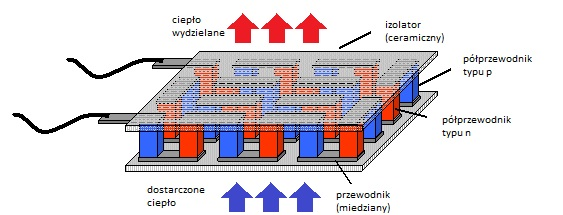
\includegraphics[scale=0.8]{budowaPeltier.jpg}
	\caption{Budowa modułu Peltiera}
\end{figure}
Półprzewodnikami wykorzystanymi do budowy ogniwa są tellurk oraz bizmut, które połączono ze sobą miedzianymi blaszkami. Istotą działania modułów Peltiera są zachodzące zmiany temperatur na połączeniach półprzewodników n-p, p-n, w wyniku przepływu prądu elektrycznego, którego wartość ma wpływ na ilość ciepła, które może zostać przetransportowana między stronami. Półprzewodnik typu n charakteryzuje się nadmiarową ilością elektronów, a typu p ich niewystarczalną ilością do wejścia na wyższy poziom energetyczny. Podczas przepływu prądu, elektrony przemieszczają się między poziomami energetycznymi, co w zależności od typu półprzewodnika oznacza zapotrzebowanie na dostarczenie energii (strona zimna) lub powoduje jej wydzielanie (strona ciepła). Niestety moduł nie jest idealny i część energii zostaje utracona w wyniku czego dochodzi również do ogrzania komponentów ogniwa.

Przydatną cechą modułów Peltiera jest możliwość połączenia ich kaskadowo tak by strona ciepła kolejnego ogniwa stykała się ze stroną zimną poprzedniego, co może pozwolić na wzrost wydajności układu. Ze względu na dużą ilość wydzielanego ciepła, zaleca się wykorzystanie pasty termoprzewodzącej oraz radiatorów po stronie ciepłej ogniwa.



\section{Arduino} %%jest OK
Arduino to sprzęt komputerowy i oprogramowanie stworzone przez firmę o tej samej nazwie, skupiające się na tworzenie zestawów uruchomieniowych opartych o mikrokontrolery z rodziny ATmega. Układ umieszczany jest na pojedynczej płytce drukowanej, z wyprowadzonymi wejściami i wyjściami układu. Język programowania  również nazywa się Arduino i został oparty o język C i C++. Najpopularniejszym ich produktem jest Arduino Uno. Wszystkie produkty wydawane są z otwartą licencją sprzętową i oprogramowania, dlatego na to na rynku dostępne są liczne klony płytek, zgodne z jej oryginalną specyfikacją. Urządzenia Arduino
może zostać wykorzystane jako samodzielny obiekt lub może być podłączone do komputera użytkownika.
\subsection{Hardware}%%jest OK
\begin{figure}[H]
	\centering
	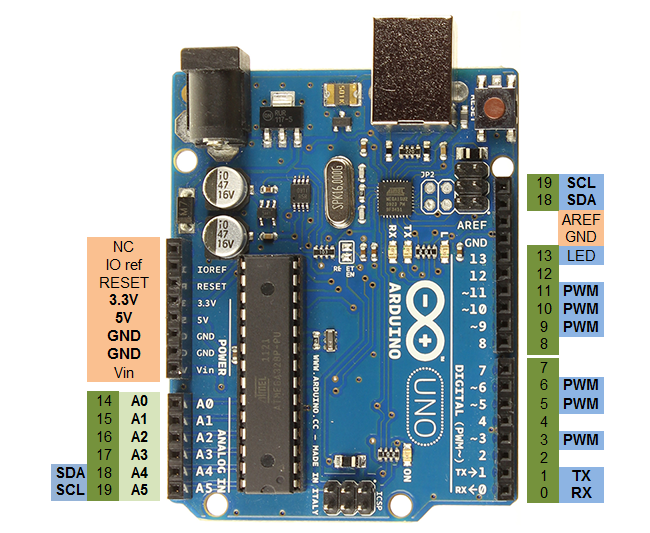
\includegraphics[scale=0.4]{ArduinoUno_pinout.png}
	\caption{Rozmieszczenie pinów dostępnych w Arduino Uno}
\end{figure}
Typowa płytka Arduino składa sie z mikrokontrolera, cyfrowych wejść/wyjść oraz wejść analogowych. Poza tym można na niej znaleźć takie interfejsy jak UART oraz USB do połączenia z komputerem, SPI i I2C do komunikacji z urządzeniami elektronicznymi.

W tej pracy wykorzystano płytkę Arduino Uno. Arduino Uno oparte jest o 8-bitowy mikrokontroler ATmega328, który uzupełniono elementami pozwalającymi na łatwiejsze programowanie wykorzystując port RS232 oraz sterowanie wyjściami mikrokontrolera. Płytka zawiera 5V regulator napięcia oraz rezonator kwarcowy o częstotliwości oscylacji 16MHz. Wyjścia mikrokontrolera zostały opisane i wyprowadzone jako żeńskie piny na obrzeżach płytki. Zastosowane rozwiązanie pozwala na łatwe podpięcie modułów rozszerzających funkcjonalność Arduino, nazywanych \textit{shieldami}. 

Arduino Uno posiada 6 wejść analogowych, 14 cyfrowych pinów wejścia/wyjścia, gdzie aż 6 z nich może zostać wykorzystane do generowania sygnału PWM. Oprócz tego można na niej znaleźć wyprowadzenia zasilania 3.3V i 5V. Piny analogowe zostały oznaczone literką A.
\newpage
\subsection{Programowanie}%%jest OK
\begin{figure}[H]
	\centering
	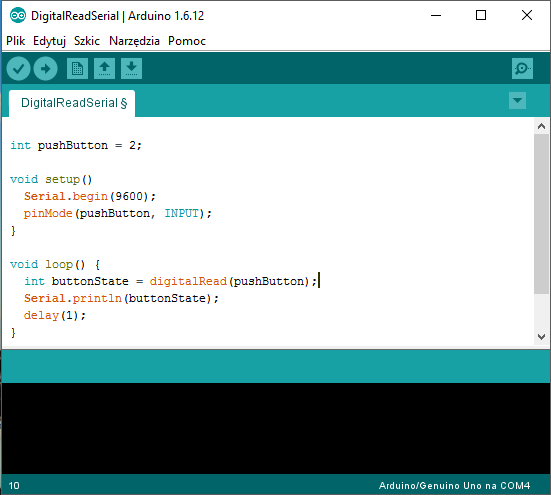
\includegraphics[scale=0.8]{pictures/arduinoIDE.PNG}
	\caption{Arduino IDE- przykładowy program}
	\label{ArduinoPodstawoweFunkcje}
\end{figure}
Do programowania płytek Arduino wykorzystuje się dedykowane oprogramowania Arduino IDE, które powstało na podstawie projektu Wiring oraz interfejs szeregowy RS232. Proces ten został ułatwiony poprzez wcześniejsze zaprogramowanie mikrokontrolera programem rozruchowym, zwalniającym z potrzeby używania zewnętrznego programatora. Oprogramowanie zawiera tak przydatne funkcje jak: kolorowanie składni kodu, automatyczne formatowanie, kompilację oraz wgrywanie programu na urządzenie docelowe. Zaletą Arduino IDE są dostępne opcje monitorowania portu szeregowego komputera w formie tekstowej, wykorzystując narzędzie ,,Monitor portu szeregowe'' oraz w postaci wykresu używając ,,Kreślarki''. Zawarta w programie biblioteka Wiring, będąca biblioteką C/C++, pozwala na ułatwienie wykonywania podstawowych operacji wejścia/wyjścia.

Aby stworzyć działający projekt należy zdefiniować dwie podstawowe funkcje:
\begin{itemize}
\item setup()- funkcja wykonywana tylko raz, wywoływana na początku programu w celu załadowania ustawień,
\item loop()- główne ciało programu, funkcja wykonywana jest wielokrotnie przez cały czas działania programu.
\end{itemize}


\section{Technologie internetowe}
\subsection{Cordova} %%jest OK
Apache Cordova to popularny framework służący do tworzenia aplikacji mobilnych w językach znanych deweloperom webowym. Cordova pozwala na utworzenie aplikacji na urządzenia mobilne wykorzystując HTML5, CSS3 oraz JavaScript. Jest to ciekawe rozwiązanie pozwalające na uniezależnienie się od środowisk programistycznych, specyficznych dla danej platformy jak np. Android Studio dla urządzeń z oprogramowaniem Android.

Cordova pozwala na napisanie jednej aplikacji, która następnie zostanie odpowiednio przetworzona, tak by działała na odpowiedniej platformie dystrybucji- urządzeniu Android lub iOS. W ten sposób uzyskuje się aplikację hybrydową, która nie jest w pełni natywna ze względu na interfejs użytkownika, który jest generowany w powłoce przeglądarki oraz nie w pełni webowa, bo zostaje skompilowana w paczkę dystrybucyjną, np. o rozszerzeniu app. Aplikacja ma dostęp do podzespołów telefonu, między innymi Bluetooth, WiFi, akcelerometr, GPS. 

\subsection{Ionic Framework}%%jest OK
Ionic to framework służący do tworzenia hybrydowych aplikacji mobilnych wykorzystujących HTML5, CSS i JavaScript. Został zbudowany z wykorzystaniem AngularJS oraz Apache Cordova. Takie rozwiązanie pozwala na dystrybucję aplikacji na różne platformy. Ionic mozna określić jako paczkę narzędzi, usług i stylów odpowiadającą za kreowanie przyjaznego interfejsu użytkownika. Jest ona odpowiednikiem wzbogaconego Bootstrapa w wersji dla aplikacji mobilnych.

Ionic zapewnia wszystkie funkcje dostępne w podstawowych SDK (zestaw narzędzi dla programistów, niezbędny w tworzeniu aplikacji na dany system) dla danej platformy. Interakcja z niestandardowymi komponentami i metodami udostępnionymi przez Ionic, możliwa jest poprzez wykorzystanie języka AngularJS.

\subsection{HTML}%%jest OK
HTML (HyperText Markup Language) to hipertekstowy język znaczników służący do tworzenia stron i aplikacji internetowych. W tej pracy wykorzystano HTML 5, który wywodzi się z języka HTML 4 i XHTML 1. Został on przyjęty za aktualny standard i jest wspierany przez wszystkie środowiska i producentów przeglądarek internetowych. Wraz z kaskadowymi arkuszami stylów i JavaScriptem tworzy on grupę najpopularniejszych technologii internetowych. HTML opisuje strukturę strony w sposób semantyczny, nadając treści dokumentu odpowiednie właściwości i funkcje, takie jak formowanie hiperłącza, list, nagłówków i akapitów. Do pozostałych funkcji tego języka należy możliwość załączania plików, plików graficznych i innych multimediów. Uzupełnieniem HTML jest CSS, który został opisany w kolejnym punkcie.

\subsection{Kaskadowe arkusze stylów}%%jest OK
Kaskadowe arkusze stylów (z ang. Cascading Style Sheets, w skrócie CSS) to język arkuszy stylów służący  do opisywania sposobu prezentacji zawartości dokumentu HTML, stron www. 
Arkusz stylów pozwala na opisanie wszystkich elementów dokumentu internetowego, takich jak: czcionka, kolor i rozmiar czcionki, interlinie, skalowanie elementów w zależności od rozmiarów otwartego okna oraz pozycjonowanie ich.

CSS został stworzony przez organizację W3C w 1996 roku w celu rozdzielenia warstwy prezentacji od warstwy danych. Uzyskane rozwiązanie pozwoliło na zwiększenie przejrzystości dokumentów HTML oraz ograniczyło ilość zmian wymaganych do wprowadzania podczas zmieniania stylu, który został wykorzystany na licznych podstronach.

\subsection{JavaScript}%%jest OK
JavaScript to dynamiczny, skryptowy język programowania wysokiego poziomu. Należy do grupy trzech najważniejszych języków, których musi się nauczyć każdy deweloper serwisów internetowych. Jest obsługiwany przez wszystkie nowoczesne przeglądarki internetowe bez potrzeby instalowania dodatkowych wtyczek. Mimo dużego podobieństwa w nazwie, języki Java i JavaScript znacznie różnią się składnią i dostępnymi bibliotekami. Język ten był wzorowany na C i przejął po nim między innymi funkcje warunkowe i pętle. W odróżnieniu od C jest to język prawie w pełni obiektowy.

Głównym zadaniem JavaScriptu jest zapewnienie interaktywności interfejsu użytkownika, czyli reakcja na wydarzenia takie jak wciśnięcie przycisku, wyświetlanie okien dialogowych, wywoływanie cyklicznych funkcji oraz aktualizowanie danych wyświetlanych na stronie. Poza tym pozwala na tworzenie ciasteczek i pobieranie informacji o przeglądarce użytkownika. JavaScript ma ograniczony dostęp do zasobów komputera użytkownika.

Do rozszerzenia funkcjonalności JavaScriptu wykorzystuje się lekkie biblioteki programistyczne takie jak jQuery, AngularJS ułatwiające manipulację obiektowym modelem dokumentu (z ang.DOM- Document Object Model), wykonywanie zapytań AJAX oraz dodawanie animacji na wyświetlanej stronie.

Skrypt JavaScript może zostać umieszczony na końcu dokumentu HTML, którego dotyczy, jednak ze względu na czytelność kodu i wymagany dostęp do niego dla wszystkich podstron, najczęściej zostaje umieszczony w osobnym pliku dodanym do projektu.

\subsection{AngularJS}%%jest OK
AngularJS to oparty na JavaScripcie, utworzony na otwartej licencji framework do tworzenia aplikacji internetowych, którego deweloperem jest Google. Głównym celem frameworka jest ułatwienie procesu deweloperskiego i testowania aplikacji poprzez wprowadzenie MVC (kontroler modelu widoku) po stronie użytkownika oraz MVVM (z ang. Model--viev--view-Model) w celu rozdzielenia kodu interfejsu od części logicznej.

AngularJS zaczyna pracę od przeszukania strony HTML w poszukiwaniu niestandardowych znaczników, które interpretuje i przypisuje do wejścia/wyjścia zmiennych wykorzystanych w JavaScipcie. Framework dopasowuje się do dokumentu HTML i rozszerza jego funkcjonalność o możliwość dynamicznego wyświetlania danych i aktualizowania widoku aplikacji, dzięki zaimplementowanemu dwukierunkowemu połączeniu między modelem i widokiem. Takie rozwiązanie pozwala znacznie ograniczyć ilość wymaganych do wykonania operacji w DOM.

Struktura programu w AngularJS składa się między innymi na zadeklarowany moduł aplikacji, kontroler i serwis.
\lstset{language=Java}
\begin{lstlisting} 
var app = angular.module('myApp', []);
app.controller('myController', function($scope) {
    $scope.firstName = "John";
    $scope.lastName = "Doe";
    $scope.personAge=myService.getAge();
})
app.service('myService', function() {
	var age=15;
    this.getAge = function () {
        return age;
    }
});
\end{lstlisting}
Zadaniem kontrolerów jest ingerowanie w interfejs użytkownika, reagowanie na wciśnięcia guzików oraz dokonywania zmian w wyświetlanych informacjach. \textit{Scope} to obiekt łączący ze sobą dane modelu i widoku. Serwisy tworzy się w celu zapewnienia funkcjonalności nie wpływającej bezpośrednio na interfejs, takiej jak np. pobieranie danych otrzymanych przez moduł Bluetooth, a następnie udostępnienie ich kontrolerowi poprzez funkcje zwracające wybrane dane.


\section{Komunikacja}
\subsection{Bluetooth}%%jest OK
Bluetooth to standard bezprzewodowej technologii wymiany danych na krótkim dystansie, pomiędzy urządzeniami typu klawiatura, komputer, bezprzewodowy głośnik, urządzenie mobilne, a w tym przypadku również Arduino. Został wymyślony przez firmę Ericsson w 1994 roku i został uznany za bezprzewodową alternatywę dla popularnego interfejsu RS232. Specyfikacja standardu Bluetooth obejmuje trzy klasy mocy nadawczej, 1-3 o zasięgu odpowiednio 100m, 10m i 1 metra w otwartej przestrzeni. W tej pracy wykorzystano moduł klasy 2, o zasięgu do 10 metrów.

Bluetooth pracuje na częstotliwości od 2402 do 2480 MHz, która jest globalnym standardem pasma częstotliwości krótkiego zasięgu dla zastosowań przemysłowych, naukowych i medycznych. Bluetooth dzieli wymieniane dane na pakiety. Każdy z nich zostaje wysłany na jeden z 79 wyznaczonych kanałów Bluetooth, których przepustowość wynosi 1 MHz. W przypadku modułów Bluetooth Low Energy o niższym poborze energii, kanałów jest jedynie 40, bo odstępy między nimi wynoszą aż 2 MHz. Protokół ten został oparty na strukturze Master-Slave. Zainicjować połączenie miedzy modułami może jedynie Master (w tym przypadku urządzenie mobilne), a Slave (moduł Bluetooth podłączony do Arduino) jedynie je zaakceptować. W tym protokole nie występuje problem z synchronizowaniem danych, dlatego że połączone ze sobą urządzenia otrzymują wspólny zegar, do którego działania zostaje dopasowany proces wysyłania i odbierania danych.

\subsection{UART}%%jest OK
UART ( z ang. Universal Asynchronous Receiver and Transmitter) to interfejs komunikacji szeregowej, szeroko wykorzystywany do przesyłania i odbierania danych asynchronicznie. Asynchroniczność oznacza, że dane są wysyłane nieregularnie. Ich początek i koniec jest oznaczony specjalnym symbolem. Interfejs UART został wykorzystany w tym projekcie do komunikacji między Arduino i modułem Bluetooth.
Procesor ATmega 328 znajdujący się na płytce Arduino Uno posiada specjalnie wyprowadzone piny portu szeregowego:
\begin{itemize}
\item{RXD- wejście szeregowe (,,Receive Data''),}
\item{TXD- wyjście szeregowe (,,Transmit Data'').}
\end{itemize}
Zaletą interfejsu UART jest posiadany przez niego bufor danych przeznaczony do tymczasowego przechowywania informacji w sytuacji, gdy są one szybko transmitowane.
Ten rodzaj transmisji danych charakteryzuje się również tym, że nadajnik i odbiornik nie posiada wspólnego sygnału zegarowego. W tym przypadku każde z urządzeń działa w takt własnego zegara. Podczas połączenia urządzeń należy pamiętać, aby oba miały ustawioną taką samą częstotliwość taktowania zegara.

\subsection{1-Wire}%%jest OK
One Wire to systemowa magistrala komunikacji elektronicznej pomiędzy urządzeniami, zapewniająca przesyłanie danych oraz zasilanie urządzenia przez pojedynczy kabel. Proces ten jest możliwy dzięki stopniowemu ładowaniu kondensatora znajdującego się w odbiorniku, a następnie wykorzystanie zgromadzonej energii do zasilenia urządzenia. Do magistrali może zostać podłączonych wiele urządzeń. Każdemu z nich przydzielany jest indywidualny adres 64-bitowy. Komunikację z urządzeniami inicjuje master, w tym przypadku mikrokontroler.

Przedstawiony protokół jest bardzo podobny do I2C, ale ze względu na wykorzystanie jedynie jednej linii danych, charakteryzuje się niższą prędkością przesyłania. Układ zazwyczaj zasilany jest napięciem o wartości 5V i służy do komunikacji pomiędzy niewielkimi urządzeniami, takimi jak np. termometr cyfrowy i mikrokontroler.



%%%%%%%%%%%%%%%%%%%%%%%%	Zastosowanie w Io
\chapter{Zastosowanie w IoT}
\section{Zastosowanie}
\section{Ocena przydatnosci}

%%%%%%%%%%%%%%%%%%%%%%%%	Podsumowanie
\chapter{Podsumowanie}
%\begin{figure}[H]
	\centering
	\includegraphics[scale=0.58]{schemat_dzialania.png}
	\caption{System pomiarowo-wykonawczy}
\end{figure}
System opisany w tym raporcie został oparty o trzy podstawowe urządzenia:
\begin{itemize}
\item urządzenie mobilne z oprogramowaniem Android,
\item Arduino Uno,
\item ogniwo Peltiera.
\end{itemize}
Za pomocą telefonu lub tabletu z modułem Bluetooth, użytkownik łączy się z system regulacji temperatury zbudowanym wokół Arduino. Aplikacja pozwala na wybór opcji związanych z regulacją, które zostają przesłane do Arduino za pomocą, komunikacji Bluetooth. Płytka Arduino interpretuje odczytane dane, następnie dokonuje pomiaru temperatury oraz oblicza sygnał sterujący PWM, za pomocą, którego zostaje wysterowane ogniwo Peltiera.

Podstawowe informacje na temat każdego z elementów przedstawiono w kolejnych sekcjach. Dokładny sposób działania wszystkich składowych opisano w poświęconych im rozdziałach.



\section{Ogniwo Peltiera} %%jest OK
Ogniwo Peltiera jest półprzewodnikowym elementem termoelektrycznym, wykorzystującym zjawisko Peltiera do przekazywania ciepła, dzięki czemu może pełnić funkcje grzejące i chłodzące.
\subsection{Efekt Peltiera} %%jest OK
Efekt Peltiera to zjawisko termoelektryczne polegające na bezpośrednim oddziaływaniu różnicy napięć na temperaturę oraz różnicy temperatury na pojawienie się napięcia. Efekt Peltiera opisuje zjawisko pojawienia się 
obiektu grzejącego i chłodzącego podczas zasilenia połączonych ze sobą różnych rodzajów przewodników, półprzewodników. Jego nazwa pochodzi od francuskiego naukowca. Zjawisko zaobserwowano po utworzeniu obwody z dwóch różnych przewodów, miedzianego i bizmutowego, które zostało następnie zasilone. Jeden z drutów nagrzewał się, a drugi ochładzał. Zimny pręt został umieszczony w odizolowanym obiekcie, w wyniku czego powstała lodówka o niskiej wydajności.

Kolejne eksperymenty Peltiera potwierdziły, że różne metale i półprzewodniki podłączone do zasilanego obwodu uzyskują właściwości przyjmowania lub oddawania energii cieplnej, co skutkuje ochładzaniem się elementu przyjmującego ciepło oraz ogrzewaniem materiału, który oddaje energię przyjętą przez element pochłaniający. Badania wykazały, że ilość przekazywanej w procesie energii, zależy od materiałów, z których wykonano części, natężenia przepływającego prądu oraz czasu jaki przepływał przez obwód. Na różnicę temperatur bezpośredni wpływ ma różnica zdolności termoelektrycznych miedzy materiałami oraz wartość natężenia prądu.

W określonej jednostce czasu, ilość pochłanianego i wydzielanego ciepła można opisać następującym wzorem:

\begin{equation}
	\Delta Q / \Delta T= \Pi _{AB} I
\end{equation}
\begin{math}
	\Pi _{AB} 
\end{math} 
-współczynnik Peltiera obwodu,	\\
\begin{math}
	\Delta Q
\end{math} 
-ciepło,	\\
\begin{math}
	\Delta T
\end{math}  
-czas,	\\
\begin{math}
	I
\end{math} 
-prąd.\\

W wyniku odwrócenia kierunku przepływu prądu przez układ, dochodzi do odwrócenia właściwości pochłaniania i oddawania energii materiałów.
Odkryte przez Peltiera właściwości pozwoliły na powstanie półprzewodnikowego modułu termoelektrycznego wykorzystanego w tej pracy, nazywanego ogniwem Peltiera. Odkrycie to zapoczątkowało późniejsze powstanie lodówek turystycznych, w których wykorzystuje się ogniwo Peltiera. Znajduje ono zastosowanie również w chłodnictwie przemysłowym i laboratoryjnym.

\subsection{Budowa ogniwa} %%jest OK
Ogniwo Peltiera zbudowane jest z dwóch równolegle położonych płytek ceramicznych, pomiędzy którymi rozłożone są naprzemiennie przewodniki typu ,,n'' oraz ,,p''. 
\begin{figure}[H]
	\centering
	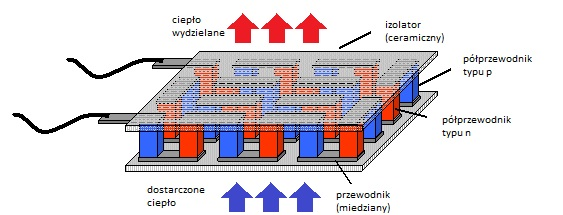
\includegraphics[scale=0.8]{budowaPeltier.jpg}
	\caption{Budowa modułu Peltiera}
\end{figure}
Półprzewodnikami wykorzystanymi do budowy ogniwa są tellurk oraz bizmut, które połączono ze sobą miedzianymi blaszkami. Istotą działania modułów Peltiera są zachodzące zmiany temperatur na połączeniach półprzewodników n-p, p-n, w wyniku przepływu prądu elektrycznego, którego wartość ma wpływ na ilość ciepła, które może zostać przetransportowana między stronami. Półprzewodnik typu n charakteryzuje się nadmiarową ilością elektronów, a typu p ich niewystarczalną ilością do wejścia na wyższy poziom energetyczny. Podczas przepływu prądu, elektrony przemieszczają się między poziomami energetycznymi, co w zależności od typu półprzewodnika oznacza zapotrzebowanie na dostarczenie energii (strona zimna) lub powoduje jej wydzielanie (strona ciepła). Niestety moduł nie jest idealny i część energii zostaje utracona w wyniku czego dochodzi również do ogrzania komponentów ogniwa.

Przydatną cechą modułów Peltiera jest możliwość połączenia ich kaskadowo tak by strona ciepła kolejnego ogniwa stykała się ze stroną zimną poprzedniego, co może pozwolić na wzrost wydajności układu. Ze względu na dużą ilość wydzielanego ciepła, zaleca się wykorzystanie pasty termoprzewodzącej oraz radiatorów po stronie ciepłej ogniwa.



\section{Arduino} %%jest OK
Arduino to sprzęt komputerowy i oprogramowanie stworzone przez firmę o tej samej nazwie, skupiające się na tworzenie zestawów uruchomieniowych opartych o mikrokontrolery z rodziny ATmega. Układ umieszczany jest na pojedynczej płytce drukowanej, z wyprowadzonymi wejściami i wyjściami układu. Język programowania  również nazywa się Arduino i został oparty o język C i C++. Najpopularniejszym ich produktem jest Arduino Uno. Wszystkie produkty wydawane są z otwartą licencją sprzętową i oprogramowania, dlatego na to na rynku dostępne są liczne klony płytek, zgodne z jej oryginalną specyfikacją. Urządzenia Arduino
może zostać wykorzystane jako samodzielny obiekt lub może być podłączone do komputera użytkownika.
\subsection{Hardware}%%jest OK
\begin{figure}[H]
	\centering
	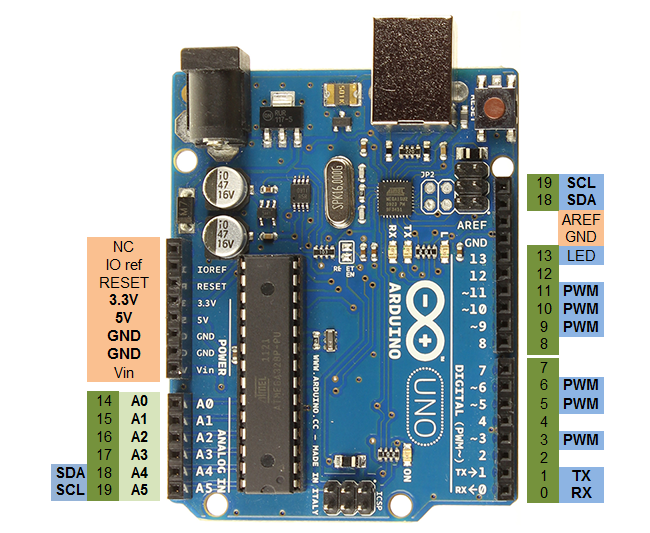
\includegraphics[scale=0.4]{ArduinoUno_pinout.png}
	\caption{Rozmieszczenie pinów dostępnych w Arduino Uno}
\end{figure}
Typowa płytka Arduino składa sie z mikrokontrolera, cyfrowych wejść/wyjść oraz wejść analogowych. Poza tym można na niej znaleźć takie interfejsy jak UART oraz USB do połączenia z komputerem, SPI i I2C do komunikacji z urządzeniami elektronicznymi.

W tej pracy wykorzystano płytkę Arduino Uno. Arduino Uno oparte jest o 8-bitowy mikrokontroler ATmega328, który uzupełniono elementami pozwalającymi na łatwiejsze programowanie wykorzystując port RS232 oraz sterowanie wyjściami mikrokontrolera. Płytka zawiera 5V regulator napięcia oraz rezonator kwarcowy o częstotliwości oscylacji 16MHz. Wyjścia mikrokontrolera zostały opisane i wyprowadzone jako żeńskie piny na obrzeżach płytki. Zastosowane rozwiązanie pozwala na łatwe podpięcie modułów rozszerzających funkcjonalność Arduino, nazywanych \textit{shieldami}. 

Arduino Uno posiada 6 wejść analogowych, 14 cyfrowych pinów wejścia/wyjścia, gdzie aż 6 z nich może zostać wykorzystane do generowania sygnału PWM. Oprócz tego można na niej znaleźć wyprowadzenia zasilania 3.3V i 5V. Piny analogowe zostały oznaczone literką A.
\newpage
\subsection{Programowanie}%%jest OK
\begin{figure}[H]
	\centering
	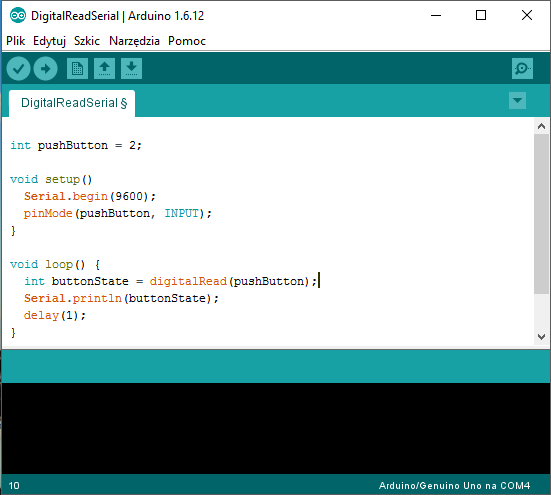
\includegraphics[scale=0.8]{pictures/arduinoIDE.PNG}
	\caption{Arduino IDE- przykładowy program}
	\label{ArduinoPodstawoweFunkcje}
\end{figure}
Do programowania płytek Arduino wykorzystuje się dedykowane oprogramowania Arduino IDE, które powstało na podstawie projektu Wiring oraz interfejs szeregowy RS232. Proces ten został ułatwiony poprzez wcześniejsze zaprogramowanie mikrokontrolera programem rozruchowym, zwalniającym z potrzeby używania zewnętrznego programatora. Oprogramowanie zawiera tak przydatne funkcje jak: kolorowanie składni kodu, automatyczne formatowanie, kompilację oraz wgrywanie programu na urządzenie docelowe. Zaletą Arduino IDE są dostępne opcje monitorowania portu szeregowego komputera w formie tekstowej, wykorzystując narzędzie ,,Monitor portu szeregowe'' oraz w postaci wykresu używając ,,Kreślarki''. Zawarta w programie biblioteka Wiring, będąca biblioteką C/C++, pozwala na ułatwienie wykonywania podstawowych operacji wejścia/wyjścia.

Aby stworzyć działający projekt należy zdefiniować dwie podstawowe funkcje:
\begin{itemize}
\item setup()- funkcja wykonywana tylko raz, wywoływana na początku programu w celu załadowania ustawień,
\item loop()- główne ciało programu, funkcja wykonywana jest wielokrotnie przez cały czas działania programu.
\end{itemize}


\section{Technologie internetowe}
\subsection{Cordova} %%jest OK
Apache Cordova to popularny framework służący do tworzenia aplikacji mobilnych w językach znanych deweloperom webowym. Cordova pozwala na utworzenie aplikacji na urządzenia mobilne wykorzystując HTML5, CSS3 oraz JavaScript. Jest to ciekawe rozwiązanie pozwalające na uniezależnienie się od środowisk programistycznych, specyficznych dla danej platformy jak np. Android Studio dla urządzeń z oprogramowaniem Android.

Cordova pozwala na napisanie jednej aplikacji, która następnie zostanie odpowiednio przetworzona, tak by działała na odpowiedniej platformie dystrybucji- urządzeniu Android lub iOS. W ten sposób uzyskuje się aplikację hybrydową, która nie jest w pełni natywna ze względu na interfejs użytkownika, który jest generowany w powłoce przeglądarki oraz nie w pełni webowa, bo zostaje skompilowana w paczkę dystrybucyjną, np. o rozszerzeniu app. Aplikacja ma dostęp do podzespołów telefonu, między innymi Bluetooth, WiFi, akcelerometr, GPS. 

\subsection{Ionic Framework}%%jest OK
Ionic to framework służący do tworzenia hybrydowych aplikacji mobilnych wykorzystujących HTML5, CSS i JavaScript. Został zbudowany z wykorzystaniem AngularJS oraz Apache Cordova. Takie rozwiązanie pozwala na dystrybucję aplikacji na różne platformy. Ionic mozna określić jako paczkę narzędzi, usług i stylów odpowiadającą za kreowanie przyjaznego interfejsu użytkownika. Jest ona odpowiednikiem wzbogaconego Bootstrapa w wersji dla aplikacji mobilnych.

Ionic zapewnia wszystkie funkcje dostępne w podstawowych SDK (zestaw narzędzi dla programistów, niezbędny w tworzeniu aplikacji na dany system) dla danej platformy. Interakcja z niestandardowymi komponentami i metodami udostępnionymi przez Ionic, możliwa jest poprzez wykorzystanie języka AngularJS.

\subsection{HTML}%%jest OK
HTML (HyperText Markup Language) to hipertekstowy język znaczników służący do tworzenia stron i aplikacji internetowych. W tej pracy wykorzystano HTML 5, który wywodzi się z języka HTML 4 i XHTML 1. Został on przyjęty za aktualny standard i jest wspierany przez wszystkie środowiska i producentów przeglądarek internetowych. Wraz z kaskadowymi arkuszami stylów i JavaScriptem tworzy on grupę najpopularniejszych technologii internetowych. HTML opisuje strukturę strony w sposób semantyczny, nadając treści dokumentu odpowiednie właściwości i funkcje, takie jak formowanie hiperłącza, list, nagłówków i akapitów. Do pozostałych funkcji tego języka należy możliwość załączania plików, plików graficznych i innych multimediów. Uzupełnieniem HTML jest CSS, który został opisany w kolejnym punkcie.

\subsection{Kaskadowe arkusze stylów}%%jest OK
Kaskadowe arkusze stylów (z ang. Cascading Style Sheets, w skrócie CSS) to język arkuszy stylów służący  do opisywania sposobu prezentacji zawartości dokumentu HTML, stron www. 
Arkusz stylów pozwala na opisanie wszystkich elementów dokumentu internetowego, takich jak: czcionka, kolor i rozmiar czcionki, interlinie, skalowanie elementów w zależności od rozmiarów otwartego okna oraz pozycjonowanie ich.

CSS został stworzony przez organizację W3C w 1996 roku w celu rozdzielenia warstwy prezentacji od warstwy danych. Uzyskane rozwiązanie pozwoliło na zwiększenie przejrzystości dokumentów HTML oraz ograniczyło ilość zmian wymaganych do wprowadzania podczas zmieniania stylu, który został wykorzystany na licznych podstronach.

\subsection{JavaScript}%%jest OK
JavaScript to dynamiczny, skryptowy język programowania wysokiego poziomu. Należy do grupy trzech najważniejszych języków, których musi się nauczyć każdy deweloper serwisów internetowych. Jest obsługiwany przez wszystkie nowoczesne przeglądarki internetowe bez potrzeby instalowania dodatkowych wtyczek. Mimo dużego podobieństwa w nazwie, języki Java i JavaScript znacznie różnią się składnią i dostępnymi bibliotekami. Język ten był wzorowany na C i przejął po nim między innymi funkcje warunkowe i pętle. W odróżnieniu od C jest to język prawie w pełni obiektowy.

Głównym zadaniem JavaScriptu jest zapewnienie interaktywności interfejsu użytkownika, czyli reakcja na wydarzenia takie jak wciśnięcie przycisku, wyświetlanie okien dialogowych, wywoływanie cyklicznych funkcji oraz aktualizowanie danych wyświetlanych na stronie. Poza tym pozwala na tworzenie ciasteczek i pobieranie informacji o przeglądarce użytkownika. JavaScript ma ograniczony dostęp do zasobów komputera użytkownika.

Do rozszerzenia funkcjonalności JavaScriptu wykorzystuje się lekkie biblioteki programistyczne takie jak jQuery, AngularJS ułatwiające manipulację obiektowym modelem dokumentu (z ang.DOM- Document Object Model), wykonywanie zapytań AJAX oraz dodawanie animacji na wyświetlanej stronie.

Skrypt JavaScript może zostać umieszczony na końcu dokumentu HTML, którego dotyczy, jednak ze względu na czytelność kodu i wymagany dostęp do niego dla wszystkich podstron, najczęściej zostaje umieszczony w osobnym pliku dodanym do projektu.

\subsection{AngularJS}%%jest OK
AngularJS to oparty na JavaScripcie, utworzony na otwartej licencji framework do tworzenia aplikacji internetowych, którego deweloperem jest Google. Głównym celem frameworka jest ułatwienie procesu deweloperskiego i testowania aplikacji poprzez wprowadzenie MVC (kontroler modelu widoku) po stronie użytkownika oraz MVVM (z ang. Model--viev--view-Model) w celu rozdzielenia kodu interfejsu od części logicznej.

AngularJS zaczyna pracę od przeszukania strony HTML w poszukiwaniu niestandardowych znaczników, które interpretuje i przypisuje do wejścia/wyjścia zmiennych wykorzystanych w JavaScipcie. Framework dopasowuje się do dokumentu HTML i rozszerza jego funkcjonalność o możliwość dynamicznego wyświetlania danych i aktualizowania widoku aplikacji, dzięki zaimplementowanemu dwukierunkowemu połączeniu między modelem i widokiem. Takie rozwiązanie pozwala znacznie ograniczyć ilość wymaganych do wykonania operacji w DOM.

Struktura programu w AngularJS składa się między innymi na zadeklarowany moduł aplikacji, kontroler i serwis.
\lstset{language=Java}
\begin{lstlisting} 
var app = angular.module('myApp', []);
app.controller('myController', function($scope) {
    $scope.firstName = "John";
    $scope.lastName = "Doe";
    $scope.personAge=myService.getAge();
})
app.service('myService', function() {
	var age=15;
    this.getAge = function () {
        return age;
    }
});
\end{lstlisting}
Zadaniem kontrolerów jest ingerowanie w interfejs użytkownika, reagowanie na wciśnięcia guzików oraz dokonywania zmian w wyświetlanych informacjach. \textit{Scope} to obiekt łączący ze sobą dane modelu i widoku. Serwisy tworzy się w celu zapewnienia funkcjonalności nie wpływającej bezpośrednio na interfejs, takiej jak np. pobieranie danych otrzymanych przez moduł Bluetooth, a następnie udostępnienie ich kontrolerowi poprzez funkcje zwracające wybrane dane.


\section{Komunikacja}
\subsection{Bluetooth}%%jest OK
Bluetooth to standard bezprzewodowej technologii wymiany danych na krótkim dystansie, pomiędzy urządzeniami typu klawiatura, komputer, bezprzewodowy głośnik, urządzenie mobilne, a w tym przypadku również Arduino. Został wymyślony przez firmę Ericsson w 1994 roku i został uznany za bezprzewodową alternatywę dla popularnego interfejsu RS232. Specyfikacja standardu Bluetooth obejmuje trzy klasy mocy nadawczej, 1-3 o zasięgu odpowiednio 100m, 10m i 1 metra w otwartej przestrzeni. W tej pracy wykorzystano moduł klasy 2, o zasięgu do 10 metrów.

Bluetooth pracuje na częstotliwości od 2402 do 2480 MHz, która jest globalnym standardem pasma częstotliwości krótkiego zasięgu dla zastosowań przemysłowych, naukowych i medycznych. Bluetooth dzieli wymieniane dane na pakiety. Każdy z nich zostaje wysłany na jeden z 79 wyznaczonych kanałów Bluetooth, których przepustowość wynosi 1 MHz. W przypadku modułów Bluetooth Low Energy o niższym poborze energii, kanałów jest jedynie 40, bo odstępy między nimi wynoszą aż 2 MHz. Protokół ten został oparty na strukturze Master-Slave. Zainicjować połączenie miedzy modułami może jedynie Master (w tym przypadku urządzenie mobilne), a Slave (moduł Bluetooth podłączony do Arduino) jedynie je zaakceptować. W tym protokole nie występuje problem z synchronizowaniem danych, dlatego że połączone ze sobą urządzenia otrzymują wspólny zegar, do którego działania zostaje dopasowany proces wysyłania i odbierania danych.

\subsection{UART}%%jest OK
UART ( z ang. Universal Asynchronous Receiver and Transmitter) to interfejs komunikacji szeregowej, szeroko wykorzystywany do przesyłania i odbierania danych asynchronicznie. Asynchroniczność oznacza, że dane są wysyłane nieregularnie. Ich początek i koniec jest oznaczony specjalnym symbolem. Interfejs UART został wykorzystany w tym projekcie do komunikacji między Arduino i modułem Bluetooth.
Procesor ATmega 328 znajdujący się na płytce Arduino Uno posiada specjalnie wyprowadzone piny portu szeregowego:
\begin{itemize}
\item{RXD- wejście szeregowe (,,Receive Data''),}
\item{TXD- wyjście szeregowe (,,Transmit Data'').}
\end{itemize}
Zaletą interfejsu UART jest posiadany przez niego bufor danych przeznaczony do tymczasowego przechowywania informacji w sytuacji, gdy są one szybko transmitowane.
Ten rodzaj transmisji danych charakteryzuje się również tym, że nadajnik i odbiornik nie posiada wspólnego sygnału zegarowego. W tym przypadku każde z urządzeń działa w takt własnego zegara. Podczas połączenia urządzeń należy pamiętać, aby oba miały ustawioną taką samą częstotliwość taktowania zegara.

\subsection{1-Wire}%%jest OK
One Wire to systemowa magistrala komunikacji elektronicznej pomiędzy urządzeniami, zapewniająca przesyłanie danych oraz zasilanie urządzenia przez pojedynczy kabel. Proces ten jest możliwy dzięki stopniowemu ładowaniu kondensatora znajdującego się w odbiorniku, a następnie wykorzystanie zgromadzonej energii do zasilenia urządzenia. Do magistrali może zostać podłączonych wiele urządzeń. Każdemu z nich przydzielany jest indywidualny adres 64-bitowy. Komunikację z urządzeniami inicjuje master, w tym przypadku mikrokontroler.

Przedstawiony protokół jest bardzo podobny do I2C, ale ze względu na wykorzystanie jedynie jednej linii danych, charakteryzuje się niższą prędkością przesyłania. Układ zazwyczaj zasilany jest napięciem o wartości 5V i służy do komunikacji pomiędzy niewielkimi urządzeniami, takimi jak np. termometr cyfrowy i mikrokontroler.




%%%%%%%%%%%%%%%%%%%%%%%%		BIBLIOGRAFIA
\addcontentsline{toc}{chapter}{Bibliografia}
\newpage
\begin{thebibliography}{99}
\bibitem{1}
\emph{Arduino Playground},
http://playground.arduino.cc/
\bibitem{seb} ktos:
\emph{tytul},
Wydawnictwo , Poznań 2000
\end{thebibliography}

\nocite{*}
\printbibliography 


%%%%%%%%%%%%%%%%%%%%%%%%		Dodatki
\chapter*{Dodatki}
\addcontentsline{toc}{chapter}{Dodatki}
Dodatek do niniejszej pracy stanowi płyta CD zawierająca:
\begin{itemize}
\item pracę dyplomową w postaci źródłowej (LaTeX),
\item pracę dyplomową w postaci pliku pdf.
\end{itemize}

\newpage
\addcontentsline{toc}{section}{Spis rysunków}	
\listoffigures

\newpage
\addcontentsline{toc}{section}{Spis tablic}	
\listoftables

%%%%%%%%%%%%%%%%%%%%%%%%

\end{document}